\section{Group -- Variable Refrigerant Flow Equipment}\label{group-variable-refrigerant-flow-equipment}

This group of EnergyPlus input objects describes the configurations of Variable Refrigerant Flow (VRF, or Variable Refrigerant Volume) air-conditioning systems.

A VRF system is an air-conditioning system that varies the refrigerant flow rate using variable speed compressor(s) in the outdoor unit, and the electronic expansion valves (EEVs) located in each indoor unit. The system meets the space cooling or heating load requirements by maintaining the zone air temperature at the setpoint. The ability to control the refrigerant mass flow rate according to the cooling and/or heating load enables the use of as many as 60 or more indoor units with differing capacities in conjunction with one single outdoor unit. This unlocks the possibility of having individualized comfort control, simultaneous heating and cooling in different zones, and heat recovery from one zone to another. It may also lead to more efficient operations during part-load conditions.

There are two alternative VRF models in EnergyPlus:

\begin{enumerate}
\def\labelenumi{\arabic{enumi}.}
\item
  \textbf{System curve based model (VRF-SysCurve)}. In this model, a number of system level curves are used to describe the VRF system performance. This model corresponds to the \emph{\hyperref[airconditionervariablerefrigerantflow]{AirConditioner:VariableRefrigerantFlow}} object.
\item
  \textbf{Physics based model (VRF-FluidTCtrl)}. This model is able to consider the dynamics of more operational parameters and is applicable for fluid temperature control. This model corresponds to the \emph{\hyperref[airconditionervariablerefrigerantflowfluidtemperaturecontrol]{AirConditioner:VariableRefrigerantFlow:FluidTemperatureControl}} object.
\end{enumerate}

(Please refer to the engineering reference for more technical details of the two models).

In the VRF system model, direct-expansion cooling and/or heating coils are configured in a zone terminal unit, which is connected to a zone via the zone inlet and exhaust nodes. The zone terminal units are identified in a \emph{\hyperref[zoneterminalunitlist]{ZoneTerminalUnitList}} object, the name of which is entered as an input to the \emph{\hyperref[airconditionervariablerefrigerantflow]{AirConditioner:VariableRefrigerantFlow}} or \emph{\hyperref[airconditionervariablerefrigerantflowfluidtemperaturecontrol]{AirConditioner:VariableRefrigerantFlow:FluidTemperatureControl}} object.

The Energyplus connection methodology is shown as dashed and greyed arrows in Figure~\ref{fig:variable-refrigerant-flow-schematic} according to the following rules:

\begin{itemize}
\item
  The zone inlet and zone exhaust node names are defined in a \emph{\hyperref[zonehvacequipmentconnections]{ZoneHVAC:EquipmentConnections}} object (bottom of figure).
\item
  A \emph{\hyperref[zonehvacterminalunitvariablerefrigerantflow]{ZoneHVAC:TerminalUnit:VariableRefrigerantFlow}} object will identify these zone exhaust and zone inlet node names as the terminal unit's air inlet and air outlet nodes, respectively.
\item
  All zone terminal units that are connected to the same \emph{\hyperref[airconditionervariablerefrigerantflow]{AirConditioner:VariableRefrigerantFlow}} or \emph{\hyperref[airconditionervariablerefrigerantflowfluidtemperaturecontrol]{AirConditioner:VariableRefrigerantFlow:FluidTemperatureControl}} object are listed in a \emph{\hyperref[zoneterminalunitlist]{ZoneTerminalUnitList}} object.
\item
  The name of the \emph{\hyperref[zoneterminalunitlist]{ZoneTerminalUnitList}} object is an input to the \emph{\hyperref[airconditionervariablerefrigerantflow]{AirConditioner:VariableRefrigerantFlow}} or \emph{\hyperref[airconditionervariablerefrigerantflowfluidtemperaturecontrol]{AirConditioner:VariableRefrigerantFlow:FluidTemperatureControl}} object.
\item
  The \emph{\hyperref[airconditionervariablerefrigerantflowfluidtemperaturecontrol]{AirConditioner:VariableRefrigerantFlow:FluidTemperatureControl}} or \emph{\hyperref[airconditionervariablerefrigerantflow]{AirConditioner:VariableRefrigerantFlow}} object is not listed in an AirloopHVAC object, and therefore, can only be simulated if the terminal units are connected to the \emph{\hyperref[airconditionervariablerefrigerantflow]{AirConditioner:VariableRefrigerantFlow}} or \emph{\hyperref[airconditionervariablerefrigerantflowfluidtemperaturecontrol]{AirConditioner:VariableRefrigerantFlow:FluidTemperatureControl}} object using the \hyperref[zoneterminalunitlist]{ZoneTerminalUnitList}.
\item
  Secondary ZoneHVAC equipment objects may be used in the same zones as the terminal units for other purposes (e.g., code compliance)
\end{itemize}

The following schematic demonstrates these connection rules.

\begin{figure}[hbtp] % fig 125
\centering
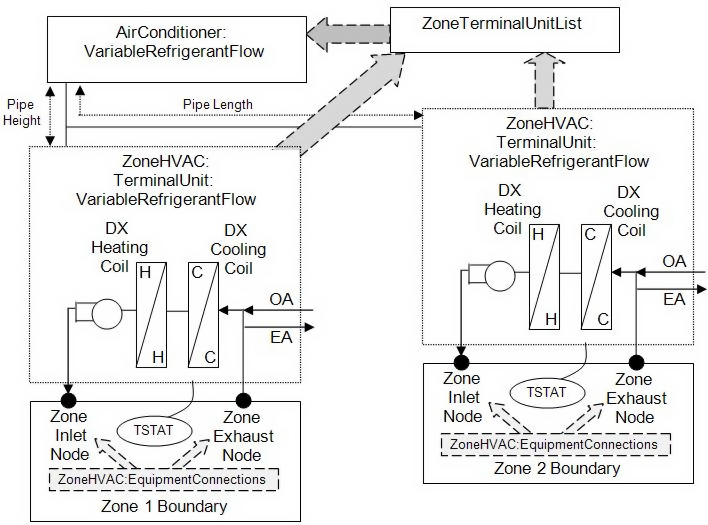
\includegraphics[width=0.9\textwidth, height=0.9\textheight, keepaspectratio=true]{media/image310.png}
\caption{Variable Refrigerant Flow Schematic \protect \label{fig:variable-refrigerant-flow-schematic}}
\end{figure}

Energyplus object type and object name, and node name relationships are also shown in the following figure to aid in the assembly of this HVAC system type.

\begin{figure}[hbtp]
\centering
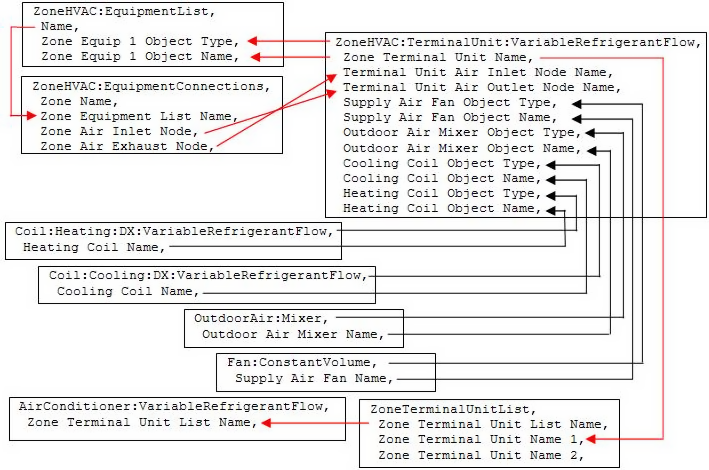
\includegraphics{media/image311.png}
\emph{(a) VRF model based on system curves (VRF-SysCurve)}

\includegraphics{media/image312.png}
\emph{(b) VRF model based on physics (VRF-FluidTCtrl)}
\caption{Variable Refrigerant Flow Object Links \protect \label{fig:variable-refrigerant-flow-object-links}}
\end{figure}

% \hyperref[airconditionervariablerefrigerantflow]{AirConditioner:VariableRefrigerantFlow}
\subsection{AirConditioner:VariableRefrigerantFlow}\label{airconditionervariablerefrigerantflow}
\subsubsection{Inputs}\label{inputs-051}

\paragraph{Field: Heat Pump Name}\label{field-heat-pump-name}

This alpha field defines a unique user-assigned name for an instance of a variable refrigerant flow heat pump. Any reference to this heat pump will use this name. Since this object is not listed in an AirloopHVAC object, the most likely use of this name would be for reporting purposes.

\paragraph{Field: Availability Schedule Name}\label{field-availability-schedule-name-018}

This alpha field defines the name of the schedule (ref: Schedule) that denotes whether the heat pump operates during a given time period. A schedule value equal to 0 denotes that the heat pump must be off for that time period. A value other than 0 denotes that the heat pump is available to operate during that time period. This schedule may be used to completely disable the heat pump (and all of its terminal units) as required. If this field is blank, the unit is enabled the entire simulation.

\paragraph{Field: Gross Rated Total Cooling Capacity}\label{field-gross-rated-total-cooling-capacity-001}

This numeric field defines the total cooling capacity (sensible + latent) of the heat pump at rated conditions in watts. The cooling capacity must be greater than 0 or set to autosize.

\paragraph{Field: Gross Rated Cooling COP}\label{field-gross-rated-cooling-cop-001}

This numeric field defines the cooling coefficient of performance at rated conditions. The cooling coefficient of performance includes compressor power and condenser fan power. This COP value does not account for impacts due to the supply air fan. The nominal heat pump cooling COP must be greater than 0. If this field is left blank, a default coefficient of performance of 3.3 is assumed.

\paragraph{Field: Minimum Outdoor Temperature in Cooling Mode}\label{field-minimum-outdoor-temperature-in-cooling-mode-000}

This numeric field defines the minimum source temperature allowed for cooling operation. For air-cooled equipment outdoor dry-bulb temperature is used. For water-cooled equipment inlet water temperature is used. Below this temperature, cooling is disabled. If this field is left blank, the default value is -6ºC.

\paragraph{Field: Maximum Outdoor Temperature in Cooling Mode}\label{field-maximum-outdoor-temperature-in-cooling-mode-000}

This numeric field defines the maximum source temperature allowed for cooling operation. For air-cooled equipment outdoor dry-bulb temperature is used. For water-cooled equipment inlet water temperature is used. Above this temperature, cooling is disabled. If this field is left blank, the default value is 43ºC.

\paragraph{Field: Cooling Capacity Ratio Modifier Function of Low Temperature Curve Name}\label{field-cooling-capacity-ratio-modifier-function-of-low-temperature-curve-name}

This alpha field defines the cooling capacity ratio modifier at low outdoor dry-bulb temperatures. This curve is a bi-quadratic equation using weighted average indoor wet-bulb temperature (i.e., the indoor terminal units weighted average inlet temperatures) and condenser entering air dry-bulb temperature as the independent variables. If the \textit{Condenser Type} is WaterCooled, then the cooling capacity modifier curve will be function of weighted average indoor air wet-bulb temperature and outdoor condenser entering water temperature. This performance curve can be used to describe the cooling capacity ratio at low outdoor temperatures (i.e., the following two curves are used) or can be used to describe the performance for all outdoor temperatures (i.e., the following two curves are not used). For this system type it is likely that all three of these performance curves will be required. See the Engineering Reference for more discussion on using this input field.

\paragraph{Field: Cooling Capacity Ratio Boundary Curve Name}\label{field-cooling-capacity-ratio-boundary-curve-name}

This alpha field defines the cooling capacity ratio boundary curve name. This curve is a linear, quadratic or cubic curve that defines a change in cooling capacity at a specific condenser entering air dry-bulb temperature as a function of indoor air wet-bulb temperature. This curve is used when the trend in cooling capacity changes dramatically as outdoor temperature changes. If the cooling capacity does not change dramatically with changes in outdoor conditions, this field may be left blank. See the Engineering Reference for more discussion on using this input field.

\paragraph{Field: Cooling Capacity Ratio Modifier Function of High Temperature Curve Name}\label{field-cooling-capacity-ratio-modifier-function-of-high-temperature-curve-name}

This alpha field defines the cooling capacity ratio modifier at high outdoor temperatures. This curve is a bi-quadratic equation using weighted average indoor wet-bulb temperature and condenser entering air dry-bulb temperature as the independent variables. This curve is used when the trend in cooling capacity changes dramatically as outdoor temperature changes. If the cooling capacity does not change dramatically with changes in outdoor conditions, this field may be left blank. See the Engineering Reference for more discussion on using this input field.

\paragraph{Field: Cooling Energy Input Ratio Modifier Function of Low Temperature Curve Name}\label{field-cooling-energy-input-ratio-modifier-function-of-low-temperature-curve-name}

This alpha field defines the cooling energy input ratio modifier at low outdoor temperatures. This curve is a bi-quadratic equation with a weighted average indoor wet-bulb temperature and condenser entering air dry-bulb temperature as the independent variables. If the \textit{Condenser Type} is WaterCooled, then the cooling energy input ratio modifier curve will be function of weighted average indoor air wet-bulb temperature and outdoor condenser entering water temperature. This performance curve can be used to describe the cooling energy input ratio at low outdoor temperatures (i.e., the following two curves are used) or can be used to describe the performance for all outdoor temperatures (i.e., the following two curves are not used). For this system type it is likely that all three of these performance curves will be required. See the Engineering Reference for more discussion on using this input field.

\paragraph{Field: Cooling Energy Input Ratio Boundary Name}\label{field-cooling-energy-input-ratio-boundary-name}

This alpha field defines the cooling energy input ratio boundary curve name. This curve is a linear, quadratic or cubic curve that defines a change in cooling energy at a specific condenser entering air dry-bulb temperature as a function of indoor air wet-bulb temperature. This curve is used when the trend in cooling energy changes dramatically as outdoor temperature changes. If the cooling energy does not change dramatically with changes in outdoor conditions, this field may be left blank. See the Engineering Reference for more discussion on using this input field.

\paragraph{Field: Cooling Energy Input Ratio Modifier Function of High Temperature Curve Name}\label{field-cooling-energy-input-ratio-modifier-function-of-high-temperature-curve-name}

This alpha field defines the cooling energy input ratio modifier at high outdoor temperatures. This curve is a bi-quadratic equation with weighted average indoor wet-bulb temperature and condenser entering air dry-bulb temperature as the independent variables. This curve is used when the trend in cooling energy changes dramatically as outdoor temperature changes. If the cooling energy does not change dramatically with changes in outdoor conditions, this field may be left blank. See the Engineering Reference for more discussion on using this input field.

\paragraph{Field: Cooling Energy Input Ratio Modifier Function of Low Part-Load Ratio Curve Name}\label{field-cooling-energy-input-ratio-modifier-function-of-low-part-load-ratio-curve-name}

This alpha field defines the cooling energy input ratio modifier (function of part-load ratio when PLR is less than or equal to 1) curve name. This curve is a linear, quadratic or cubic equation with cooling part-load ratio used as the independent variable. The cooling energy input ratio modifier curve is normalized to 1 at a part-load ratio of 1 and is used only when the operating part-load ratio is less than or equal to 1.

\paragraph{Field: Cooling Energy Input Ratio Modifier Function of HIgh Part-Load Ratio Curve Name}\label{field-cooling-energy-input-ratio-modifier-function-of-high-part-load-ratio-curve-name}

This alpha field defines the cooling energy input ratio modifier (function of part-load ratio when PLR is greater than 1) curve name. This curve is a linear, quadratic or cubic equation with cooling part-load ratio used as the independent variable. The cooling energy input ratio modifier curve is normalized to 1 at a part-load ratio of 1 and is used only when the operating part-load ratio is greater than 1.

\paragraph{Field: Cooling Combination Ratio Correction Factor Curve Name}\label{field-cooling-combination-ratio-correction-factor-curve-name}

This alpha field defines the cooling combination ratio (CR) correction factor curve name for combination ratios greater than or equal to 1. The combination ratio is defined as the total rated indoor terminal unit cooling capacity divided by this heat pump's gross rated total cooling capacity. The curve is a linear, quadratic or cubic equation and uses the minimum value of x in the curve object to determine the maximum part-load ratio which is linearly proportional to capacity (i.e., the minimum value of x {[}CR{]} in the curve object must be ≥1). The output of this curve provides a multiplier (\textgreater{}1) which is applied to this heat pump's Gross Rated Total Cooling Capacity. Between a combination ratio of 1 and the curve's minimum value of x, the multiplier is linearly interpolated. For combination ratio's less than 1 (i.e., the total indoor terminal unit capacity is less than this heat pump's rated total capacity), capacity is directly proportional to part-load ratio and this curve will not be used.

\paragraph{Field: Cooling Part-Load Fraction Correlation Curve Name}\label{field-cooling-part-load-fraction-correlation-curve-name}

This alpha field defines the cooling part-load fraction correlation curve name. This curve is used to define the cycling losses when the condenser's compressors cycle on and off. The compressor cycles when the cooling part-load ratio is less than the Minimum Heat Pump Part-Load Ratio specified later in this object's inputs.

\paragraph{Field: Gross Rated Heating Capacity}\label{field-gross-rated-heating-capacity-001}

This numeric field defines the gross total heat pump heating capacity at rated conditions in watts. The nominal heat pump heating capacity must be greater than 0 or set to autosize.

\paragraph{Field: Rated Heating Capacity Sizing Ratio}\label{field-rated-heating-capacity-sizing-ratio-000}

This numeric field defines the ratio of gross heating to gross cooling capacity. The model assumes that when used, this value will be greater than 1. A similar input is available in the \hyperref[zonehvacterminalunitvariablerefrigerantflow]{ZoneHVAC:TerminalUnit:VariableRefrigerantFlow} object. When the heating capacity is autosized, if this field is non-blank, this ratio is used to scale the heating capacity to the gross rated total cooling capacity regardless of the value entered in the terminal unit objects. When the heating capacity is not autosized, the gross rated heating capacity will be equal to the value specified in the Gross Rated Heating Capacity input field and this value will be compared to the sum of the terminal unit heating coil size. If these values are more than 10\% different, a warning will be issued when \hyperref[outputdiagnostics]{Output:Diagnostics}, DisplayExtraWarnings; is included in the input file. If this field is blank and the terminal unit sizing ratio input is also blank, then the heating capacity sizing ratio is assumed to be 1. If this field is not blank and the heating capacity sizing ratio in the terminal unit object(s) is blank, then this ratio also applies to each heating coil. If this field is not blank and the heating capacity sizing ratio in the terminal units is also not blank, then the terminal unit heating coil capacity sizing ratio input applies to each heating coil.

\paragraph{Field: Gross Rated Heating COP}\label{field-gross-rated-heating-cop-001}

This numeric field defines the heating coefficient of performance at rated conditions. The heating coefficient of performance includes compressor power and condenser fan power. This gross COP value does NOT account for~ the supply air fan. The nominal heat pump heating COP must be greater than 0. If this field is left blank, a coefficient of performance of 3.4 is assumed.

\paragraph{Field: Minimum Outdoor Temperature in Heating Mode}\label{field-minimum-outdoor-temperature-in-heating-mode-000}

This numeric field defines the minimum outdoor temperature allowed for heating operation. Below this temperature, heating is disabled. If this field is left blank, the default value is -20ºC.

\paragraph{Field: Maximum Outdoor Temperature in Heating Mode}\label{field-maximum-outdoor-temperature-in-heating-mode-000}

This numeric field defines the maximum outdoor temperature allowed for heating operation. Above this temperature, heating is disabled. If this field is left blank, the default value is 16ºC.

\paragraph{Field: Heating Capacity Ratio Modifier Function of Low Temperature Curve Name}\label{field-heating-capacity-ratio-modifier-function-of-low-temperature-curve-name}

This alpha field defines the heating capacity ratio modifier at low temperature curve name. This curve is a bi-quadratic equation with a weighted average indoor dry-bulb temperature (i.e., the indoor terminal units weighted average inlet temperatures) and condenser entering air dry-bulb or wet-bulb temperature as the independent variables. Since manufacturers may provide performance data using either outdoor dry-bulb or wet-bulb temperatures, either of these temperature types may be used for heating performance curves as specified in the Heating Performance Curve Outdoor Temperature Type input field below. This performance curve can be used to describe the heating capacity ratio at low outdoor temperatures (i.e., the following two curves are used) or can be used to describe the performance for all outdoor temperatures (i.e., the following two curves are not used). For this system type it is likely that all three of these performance curves will be required. See the Engineering Reference for more discussion on using this input field.

\paragraph{Field: Heating Capacity Ratio Boundary Curve Name}\label{field-heating-capacity-ratio-boundary-curve-name}

This alpha field defines the heating capacity ratio boundary curve name. This curve is a quadratic or cubic curve that defines a change in heating capacity at a specific condenser entering air dry-bulb or wet-bulb temperature as a function of indoor air dry-bulb temperature. Since manufacturers may provide performance data using either outdoor dry-bulb or wet-bulb temperatures, either of these temperature types may be used for heating performance curves as specified in the Heating Performance Curve Outdoor Temperature Type input field below. This curve is used when the trend in heating capacity changes dramatically as outdoor temperature changes. If the heating capacity does not change dramatically with changes in outdoor conditions, this field may be left blank.

\paragraph{Field: Heating Capacity Ratio Modifier Function of High Temperature Curve Name}\label{field-heating-capacity-ratio-modifier-function-of-high-temperature-curve-name}

This alpha field defines the heating capacity ratio modifier at high temperature curve name. This curve is a bi-quadratic equation with a weighted average indoor dry-bulb temperature and condenser entering air dry-bulb or wet-bulb temperature as the independent variables. Since manufacturers may provide performance data using either outdoor dry-bulb or wet-bulb temperatures, either of these temperature types may be used for heating performance curves as specified in the Heating Performance Curve Outdoor Temperature Type input field below. This curve is used when the trend in heating capacity changes dramatically as outdoor temperature changes. If the heating capacity does not change dramatically with changes in outdoor conditions, this field may be left blank.

\paragraph{Field: Heating Energy Input Ratio Modifier Function of Low Temperature Curve Name}\label{field-heating-energy-input-ratio-modifier-function-of-low-temperature-curve-name}

This alpha field defines the heating energy input ratio modifier at low temperature curve name. This curve is a bi-quadratic equation with a weighted average indoor dry-bulb temperature and condenser entering air dry-bulb or wet-bulb temperature as the independent variables. Since manufacturers may provide performance data using either outdoor dry-bulb or wet-bulb temperatures, either of these temperature types may be used for heating performance curves as specified in the Heating Performance Curve Outdoor Temperature Type input field below. This performance curve can be used to describe the heating energy input ratio at low outdoor temperatures (i.e., the following two curves are used) or can be used to describe the performance for all outdoor temperatures (i.e., the following two curves are not used).

\paragraph{Field: Heating Energy Input Ratio Boundary Curve Name}\label{field-heating-energy-input-ratio-boundary-curve-name}

This alpha field defines the heating energy input ratio boundary curve name. This curve is a quadratic or cubic curve that defines a change in heating energy at a specific condenser entering air dry-bulb or wet-bulb temperature as a function of indoor air dry-bulb temperature. Since manufacturers may provide performance data using either outdoor dry-bulb or wet-bulb temperatures, either of these temperature types may be used for heating performance curves as specified in the Heating Performance Curve Outdoor Temperature Type input field below. This curve is used when the trend in heating energy changes dramatically as outdoor temperature changes. If the heating energy does not change dramatically with changes in outdoor conditions, this field may be left blank.

\paragraph{Field: Heating Energy Input Ratio Modifier Function of High Temperature Curve Name}\label{field-heating-energy-input-ratio-modifier-function-of-high-temperature-curve-name}

This alpha field defines the heating energy input ratio modifier at high temperature curve name. This curve is a bi-quadratic equation with a weighted average indoor dry-bulb temperature and condenser entering air dry-bulb or wet-bulb temperature as the independent variables. Since manufacturers may provide performance data using either outdoor dry-bulb or wet-bulb temperatures, either of these temperature types may be used for heating performance curves as specified in the Heating Performance Curve Outdoor Temperature Type input field below. This curve is used when the trend in heating energy changes dramatically as outdoor temperature changes. If the heating energy does not change dramatically with changes in outdoor conditions, this field may be left blank.

\paragraph{Field: Heating Performance Curve Outdoor Temperature Type}\label{field-heating-performance-curve-outdoor-temperature-type}

This choice field defines the outdoor temperature type used for all performance curves. The valid choices are DryBulbTemperature and WetBulbTemperature. The default value is WetBulbTemperature. Manufacturers will typically provide heating performance data as a function of outdoor air wet-bulb temperatures. This means that the performance (e.g., capacity and energy input ratio) curves will use outdoor wet-bulb temperature as one of the independent variables. At times, manufacturers will only provide performance data as a function of outdoor dry-bulb temperatures. In this case, all performance curves shall be developed using outdoor dry-bulb temperature and this field shall be selected as DryBulbTemperature.

\paragraph{Field: Heating Energy Input Ratio Modifier Function of Low Part-Load Ratio Curve Name}\label{field-heating-energy-input-ratio-modifier-function-of-low-part-load-ratio-curve-name}

This alpha field defines the heating energy input ratio modifier (function of part-load ratio when PLR is less than or equal to 1) curve name. This curve is a linear, quadratic, or cubic equation with heating part-load ratio used as the independent variable. The heating energy input ratio modifier curve is normalized to 1 at a part-load ratio of 1 and is used only when the part-load ratio is less than or equal to 1.

\paragraph{Field: Heating Energy Input Ratio Modifier Function of High Part-Load Ratio Curve Name}\label{field-heating-energy-input-ratio-modifier-function-of-high-part-load-ratio-curve-name}

This alpha field defines the heating energy input ratio modifier (function of part-load ratio when PLR is greater than 1) curve name. This curve is a linear, quadratic, or cubic equation with heating part-load ratio used as the independent variable. The heating energy input ratio modifier curve is normalized to 1 at a part-load ratio of 1 and is used only when the part-load ratio is greater than 1.

\paragraph{Field: Heating Combination Ratio Correction Factor Curve Name}\label{field-heating-combination-ratio-correction-factor-curve-name}

This alpha field defines the heating combination ratio (CR) correction factor curve name for combination ratios greater than or equal to 1. The combination ratio is defined as the total rated indoor heating capacity divided by the rated heat pump heating capacity. The curve is either quadratic or cubic and uses the minimum value of x in the curve object to determine the maximum part-load ratio which is linearly proportional to capacity (i.e., the minimum value of x in the curve object must be ≥1). The output of this curve provides a multiplier (\textgreater{}1) which is applied to the Nominal Heat Pump Heating Capacity. Between a combination ratio of 1 and the curve's minimum value of x, the multiplier is linearly interpolated. For combination ratio's less than 1, capacity is directly proportional to part-load ratio and this curve will not be used. If this field is left blank, the Cooling Combination Ratio Correction factor will be used.

\paragraph{Field: Heating Part-Load Fraction Correlation Curve Name}\label{field-heating-part-load-fraction-correlation-curve-name}

This alpha field defines the heating part-load fraction correlation curve name. This curve is used to define the cycling losses when the condenser's compressors cycle on and off. The compressor cycles when the indoor to outdoor heating capacity ratio is less than the Minimum Heat Pump Part-Load Ratio specified in the following field.

\paragraph{Field: Minimum Heat Pump Part-Load Ratio}\label{field-minimum-heat-pump-part-load-ratio-000}

This numeric field specifies the minimum operating part-load ratio (PLR) of the heat pump. When the heat pump operates at a PLR below this value, the heat pump's compressor will cycle to meet the cooling or heating demand. Above this value, the heat pump's compressor operates the entire time step to meet the cooling or heating demand. The minimum value for this field is 0. If this field is left blank, the default value is 0.15. When the heat pump compressor cycles, the previous field is used to determine cycling losses.

\paragraph{Field: Zone Name for Master Thermostat Location}\label{field-zone-name-for-master-thermostat-location-000}

This alpha field defines the name of the zone where the ``master'' thermostat is located. When the heat pump is connected to multiple zone terminal units, one terminal unit must be selected as the master thermostat. The remaining thermostats are slaves and can operate only in the same mode as the master thermostat.

\paragraph{Field: Master Thermostat Priority Control Type}\label{field-master-thermostat-priority-control-type-000}

This choice field determines the logic used to simulate the ``master'' thermostat. Valid choices are LoadPriority, ZonePriority, ThermostatOffsetPriority, MasterThermostatPriority, and Scheduled. The default value is MasterThermostatPriority. When LoadPriority is selected, the total zone load is used to choose the operating mode as either cooling or heating. When ZonePriority is selected, the number of zones requiring cooling or heating determines the operating mode. When ThermostatOffsetPriority is selected, the zone farthest from the thermostat set point determines the operating mode. The MasterThermostatPriority choice operates the system according the zone load where the master thermostat is located. The heat pump can also be scheduled to operate in either cooling or heating mode. For scheduled operation, a schedule name is entered in the following field.

\paragraph{Field: Thermostat Priority Schedule Name}\label{field-thermostat-priority-schedule-name-000}

This alpha field identifies the schedule used when the previous field is set to Scheduled. Schedule values of 0 denote heating mode while values of 1 denote cooling mode. Any other values will force the system off.

\paragraph{Field: Zone Terminal Unit List Name}\label{field-zone-terminal-unit-list-name}

This alpha field defines the name of the zone terminal unit list. The name specified here should match the name of a valid \hyperref[zoneterminalunitlist]{ZoneTerminalUnitList} object. In addition, each name specified in this list should match the name of a valid ZoneHVAC:TerminalUnit: VariableRefrigerantFlow object. All terminal units connected to this heat pump must be listed in this \hyperref[zoneterminalunitlist]{ZoneTerminalUnitList} object.

Note: the previous field is designated at the last field necessary to simulate the variable refrigerant flow heat pump. The following fields do not have to be entered, however, piping loses, defrost operation, crankcase heater operation, and basin heater operation will not be modeled. Defaults for fields not entered may also not apply. These remaining fields must be entered if that portion of the model is to be simulated.

\paragraph{Field: Heat Pump Waste Heat Recovery}\label{field-heat-pump-waste-heat-recovery-000}

This choice field defines the configuration of the heat pump refrigeration system. Valid choices are \textbf{Yes} and \textbf{No}. If Yes is selected, heat recovery is enabled and the heat pump can independently cool and heat different zones. If No is selected, the heat pump is only able to cool or heat for any given time step.

\paragraph{Field: Equivalent Piping Length used for Piping Correction Factor in Cooling Mode}\label{field-equivalent-piping-length-used-for-piping-correction-factor-in-cooling-mode-000}

This numeric field defines the equivalent pipe length in meters between the farthest terminal unit and the heat pump condenser. This value includes the gas refrigerant line length (for both horizontal and vertical distances), fitting losses, pipe bends, and other connections that contribute to piping losses. This field is used to calculate the piping correction factor in cooling mode. This value defines the head losses due to the pipe length between the farthest terminal unit and the heat pump condenser and impacts the maximum available capacity in cooling mode.

\paragraph{Field: Vertical Height used for Piping Correction Factor}\label{field-vertical-height-used-for-piping-correction-factor-000}

This numeric field defines the vertical pipe height in meters between the highest or lowest terminal unit and the heat pump condenser. This value defines the gravitational losses due to a change in height between the highest (positive value), or lowest (negative value) terminal unit and the heat pump condenser. The distance specified here is applied to the piping correction factor calculation for both cooling and heating. If the distance between the highest terminal unit above the heat pump condenser is greater than the distance between the lowest terminal unit below the condenser enter the difference between the highest and lowest terminal units as a positive distance, otherwise enter this difference as a negative distance. Example: if the distance from the heat pump condenser to the highest terminal unit above the condenser is 10 m and the distance from the heat pump condenser to the lowest terminal unit below the condenser is -15 m, then enter a value of -5 m in this field. This head loss impacts the maximum available capacity in cooling mode.

\paragraph{Field: Piping Correction Factor for Length in Cooling Mode Curve Name}\label{field-piping-correction-factor-for-length-in-cooling-mode-curve-name}

This alpha field defines the linear, quadratic, or cubic curve name used to calculate the piping correction factor for length in cooling mode. Piping losses are a function of piping length. If sufficient piping loss information is available where piping losses are also a function of combination ratio (i.e., in addition to length), a biquadratic performance curve may be used.

\paragraph{Field: Piping Correction Factor for Height in Cooling Mode Coefficient}\label{field-piping-correction-factor-for-height-in-cooling-mode-coefficient}

This numeric field defines the coefficient used to calculate the piping correction factor for height in cooling mode.

\paragraph{Field: Equivalent Piping Length used for Piping Correction Factor in Heating Mode}\label{field-equivalent-piping-length-used-for-piping-correction-factor-in-heating-mode-000}

This numeric field defines the equivalent pipe length in meters between the farthest terminal unit and the heat pump condenser. This value includes the liquid refrigerant line length (for both horizontal and vertical distances), fitting losses, pipe bends, and other connections that contribute to piping losses. This field is used to calculate the piping correction factor in heating mode. This value defines the head losses due to the pipe length between the farthest terminal unit and the heat pump condenser and impacts the maximum available capacity in heating mode.

\paragraph{Field: Piping Correction Factor for Length in Heating Mode Curve Name}\label{field-piping-correction-factor-for-length-in-heating-mode-curve-name}

This alpha field defines the linear, quadratic, or cubic curve name used to calculate the piping correction factor for length in heating mode. Piping losses are a function of piping length. If sufficient piping loss information is available where piping losses are also a function of combination ratio (i.e., in addition to length), a biquadratic performance curve may be used.

\paragraph{Field: Piping Correction Factor for Height in Heating Mode Coefficient}\label{field-piping-correction-factor-for-height-in-heating-mode-coefficient}

This numeric field defines the coefficient used to calculate the piping correction factor for height in heating mode.

\paragraph{Field: Crankcase Heater Power per Compressor}\label{field-crankcase-heater-power-per-compressor-000}

This numeric field defines the electrical power consumed by the crankcase heater in watts for \emph{each} compressor. This crankcase heater power is consumed when the outdoor temperature is below the maximum outdoor dry-bulb temperature for crankcase heater operation. The minimum value for this field is 0. If this field is left blank, the default value is 33 watts. Crankcase heater electrical consumption is applied only when the compressor is off or is applied during the off cycle when the compressor is cycling below the Minimum Heat Pump Part-Load Ratio. This field is only used to calculate crankcase heater power and has no impact on heat pump performance.

\paragraph{Field: Number of Compressors}\label{field-number-of-compressors-000}

This numeric field defines the number of compressors in the heat pump condensing unit and is used exclusively to determine the operating characteristics of the crankcase heater. For example, if the number of compressors is 3, one crankcase heater will operate when the heat pump condensing unit's part-load ratio is less than or equal to 0.67 (when the ratio of compressor size to total compressor capacity input is 0.33) and the outdoor temperature is below the maximum outdoor temperature for crankcase heater operation. Similarly, two crankcase heaters will operate when the heat pump condensing unit's PLR is less than or equal to 0.33 and the outdoor temperature is below the maximum outdoor temperature for crankcase heater operation. If the heat pump condensing unit is off, all 3 crankcase heaters will operate if the outdoor temperature is below the maximum outdoor temperature for crankcase heater operation. The minimum value for this field is 1. If this field is left blank, the default value is 2. This field is only used to calculate crankcase heater power and has no impact on heat pump performance.

\paragraph{Field: Ratio of Compressor Size to Total Compressor Capacity}\label{field-ratio-of-compressor-size-to-total-compressor-capacity-000}

This numeric field defines the size of the first stage compressor to the total compressor capacity and is used exclusively for calculating crankcase heater energy. If this field and the previous field are left blank, the default value is 0.5.~ If this field is left blank and the previous field is not blank, the compressors are assumed to be equally sized. When the number of compressors is greater than 2, the 2\(^{nd}\) stage compressor and all additional compressors are assumed to be equally sized. This field is only used to calculate crankcase heater power and has no impact on heat pump performance.

\paragraph{Field: Maximum Outdoor Dry-bulb Temperature for Crankcase Heater}\label{field-maximum-outdoor-dry-bulb-temperature-for-crankcase-heater-000}

This numeric field defines the maximum outdoor temperature, in degrees Celsius, below which the crankcase heater will operate. If this field is left blank, the default value is 0°C. This field is only used to calculate crankcase heater power and has no impact on heat pump performance.

\paragraph{Field: Defrost Strategy}\label{field-defrost-strategy-001}

This alpha field has two choices: reverse-cycle or resistive. If the reverse-cycle strategy is selected, the heating cycle is reversed periodically to provide heat to melt frost accumulated on the outdoor coil. If a resistive defrost strategy is selected, the frost is melted using an electric resistance heater. If this input field is left blank, the default defrost strategy is reverse-cycle. Defrost can be disabled by entering a resistive defrost strategy using a timed defrost control, a 0 defrost time period fraction and a 0 resistive defrost heater capacity in the following inputs fields. This method is used when the Maximum Outdoor Dry-Bulb Temperature for Defrost Operation field value is greater than the expected minimum outdoor dry-bulb temperature simulated in the weather file.

\paragraph{Field: Defrost Control}\label{field-defrost-control-001}

This alpha field has two choices: timed or on-demand. If timed control is selected, the defrost time period is calculated based on a fixed value of compressor runtime whether or not frost has actually accumulated. For timed defrost control, the fractional amount of time the unit is in defrost is entered in the input field ``Defrost Time Period Fraction'' described below. If on-demand defrost control is selected, the defrost time period is calculated based on outdoor weather (humidity ratio) conditions. Regardless of which defrost control is selected, defrost does not occur above the user specified outdoor temperature entered in the input field ``Maximum Outdoor Dry-bulb Temperature for Defrost Operation'' described above. If this input field is left blank, the default defrost control is timed.

\paragraph{Field: Defrost Energy Input Ratio Modifier Function of Temperature Curve Name}\label{field-defrost-energy-input-ratio-modifier-function-of-temperature-curve-name}

This alpha field defines the name of a bi-quadratic performance curve (ref: Performance Curves) that parameterizes the variation of the energy input ratio (EIR) during reverse-cycle defrost periods as a function of the weighted average wet-bulb temperature of the air entering the indoor terminal units (variable x) and the outdoor air dry-bulb temperature (variable y). The output of this curve is multiplied by the coil capacity, the fractional defrost time period and the runtime fraction of the heating coil to give the defrost power at the specific temperatures at which the indoor and outdoor coils are operating. The curve is normalized to a value of 1.0 at the rating point conditions.

\paragraph{Field: Defrost Time Period Fraction}\label{field-defrost-time-period-fraction-001}

This numeric field defines the fraction of compressor runtime when the defrost cycle is active. For example, if the defrost cycle is active for 3.5 minutes for every 60 minutes of compressor runtime, then the user should enter 3.5/60 = 0.058333. The value for this input field must be greater than or equal to 0. If this input field is left blank, the default value is 0.058333.

\paragraph{Field: Resistive Defrost Heater Capacity}\label{field-resistive-defrost-heater-capacity-001}

This numeric field defines the capacity of the resistive defrost heating element in Watts. This input field is used only when the selected defrost strategy is `resistive' (see input field ``Defrost Strategy'' above). The value for this input field must be greater than or equal to 0. If this input field is left blank, the default value is 0.

\paragraph{Field: Maximum Outdoor Dry-bulb Temperature for Defrost Operation}\label{field-maximum-outdoor-dry-bulb-temperature-for-defrost-operation-001}

This numeric field defines the outdoor air dry-bulb temperature above which outdoor coil defrosting is disabled. If this input field is left blank, the default value is 5 C. Defrost can be completely eliminated by selecting a temperature lower than the minimum expected outdoor temperature found in the weather file.

\paragraph{Field: Condenser Type}\label{field-condenser-type-003}

This choice field defines the configuration of the heat pump condenser. Valid choices are \textbf{AirCooled}, \textbf{EvaporativelyCooled}, and \textbf{WaterCooled}.

\paragraph{Field: Condenser Inlet Node Name}\label{field-condenser-inlet-node-name-000}

This alpha field defines the name of the condenser inlet air or water node. For Condenser type = AirCooled, this node name should also be listed in an \hyperref[outdoorairnode]{OutdoorAir:Node} or \hyperref[outdoorairnodelist]{OutdoorAir:NodeList} object. If this field is blank, the model assumes an air-cooled condenser and the weather file is used to define the outdoor conditions entering the condenser. If this field is not blank, the node conditions are used to define the outdoor air or inlet water conditions entering the condenser. A node name is typically entered here for air-cooled systems when conditions other than those found in the weather file should be used (ref. \hyperref[outdoorairnode]{OutdoorAir:Node} related to height above ground).

\paragraph{Field: Condenser Outlet Node Name}\label{field-condenser-outlet-node-name-000}

This alpha field defines the name of the condenser outlet water node. This field is only used for water-cooled systems.

\paragraph{Field: Water Condenser Volume Flow Rate}\label{field-water-condenser-volume-flow-rate-000}

This numeric field defines the condenser water volume flow rate in cubic meters per second. This field is autosizable and only used for water-cooled systems.

\paragraph{Field: Evaporative Condenser Effectiveness}\label{field-evaporative-condenser-effectiveness-002}

The effectiveness of the evaporative condenser, which is used to determine the temperature of the air entering the outdoor condenser coil as follows:

\begin{equation}
Tcond\,inlet = \,\left( {Twb,o} \right)\,\, + \,\,\left( {1 - EvapCondEffectiveness} \right)\left( {Tdb,o\,\, - Twb,o} \right)
\end{equation}

where

\emph{T\(_{cond\\ inlet}\)} = the temperature of the air entering the condenser coil (C)

\emph{T\(_{wb,o}\)} = the wet-bulb temperature of the outdoor air (C)

\emph{T\(_{db,o}\)} = the dry-bulb temperature of the outdoor air (C)

The resulting condenser inlet air temperature is used by the Cooling Capacity Ratio Modifier Curve (function of temperature) and the Cooling Energy Input Ratio Modifier Curve (function of temperature). The default value for this field is 0.9, although valid entries can range from 0.0 to 1.0. This field is not used when Condenser Type = Air Cooled and the simulation is calculating heating performance.

If the user wants to model an air-cooled condenser, they should simply specify AirCooled in the field Condenser Type. In this case, the Cooling Capacity Ratio Modifier Curve (function of temperature) and the Cooling Energy Input Ratio Modifier Curve (function of temperature) input fields for this object should reference performance curves that are a function of outdoor dry-bulb temperature.

If the user wishes to model an evaporative-cooled condenser AND they have performance curves that are a function of the wet-bulb temperature of air entering the condenser coil, then the user should specify Condenser Type = EvapCooled and the evaporative condenser effectiveness value should be entered as 1.0. In this case, the Cooling Capacity Ratio Modifier Curve (function of temperature) and the Cooling Energy Input Ratio Modifier Curve (function of temperature) input fields for this object should reference performance curves that are a function of the wet-bulb temperature of air entering the condenser coil.

If the user wishes to model an air-cooled condenser that has evaporative media placed in front of it to cool the air entering the condenser coil, then the user should specify Condenser Type = EvapCooled. The user must also enter the appropriate evaporative effectiveness for the media. In this case, the Cooling Capacity Ratio Modifier Curve (function of temperature) and the Cooling Energy Input Ratio Modifier Curve (function of temperature) input fields for this object should reference performance curves that are a function of outdoor dry-bulb temperature. Be aware that the evaporative media will significantly reduce the dry-bulb temperature of the air entering the condenser coil, so the Cooling Capacity and Cooling EIR Modifier Curves must be valid for the expected range of dry-bulb temperatures that will be entering the condenser coil.

\paragraph{Field: Evaporative Condenser Air Flow Rate}\label{field-evaporative-condenser-air-flow-rate-002}

The air volume flow rate, in m\(^{3}\) per second, entering the evaporative condenser. This value is used to calculate the amount of water used to evaporatively cool the condenser inlet air. The minimum value for this field must be greater than zero, and this input field is autosizable (equivalent to 0.000144 m\(^{3}\)/s per watt of rated total cooling capacity {[}850 cfm/ton{]}). This field is not used when Condenser Type = AirCooled.

\paragraph{Field: Evaporative Condenser Pump Rated Power Consumption}\label{field-evaporative-condenser-pump-rated-power-consumption-001}

The rated power of the evaporative condenser water pump in Watts. This value is used to calculate the power required to pump the water used to evaporatively cool the condenser inlet air. The default value for this input field is zero, but it is autosizable (equivalent to 0.004266 W per watt {[}15 W/ton{]} of rated total cooling capacity). This field is not used when Condenser Type = AirCooled.

\paragraph{Field: Supply Water Storage Tank Name}\label{field-supply-water-storage-tank-name-001}

This alpha field defines the name of the water storage tank when an evaporatively-cooled condenser is used.

\paragraph{Field: Basin Heater Capacity}\label{field-basin-heater-capacity-004}

This numeric field contains the capacity of the heat pump's electric basin heater in watts per degree Kelvin. This field only applies for Condenser Type = EvaporativelyCooled. This field is used in conjunction with the Basin Heater Setpoint Temperature described in the following field. The basin heater electric power is equal to this field multiplied by the difference between the basin heater set point temperature and the outdoor dry-bulb temperature. The basin heater only operates when the heat pump compressor(s) is off, regardless of the basin heater schedule described below. The basin heater capacity must be greater than or equal to zero, with a default value of zero if this field is left blank.

\paragraph{Field: Basin Heater Setpoint Temperature}\label{field-basin-heater-setpoint-temperature-004}

This numeric field contains the set point temperature (˚C) for the basin heater described in the previous field. This field only applies for Condenser Type = EvaporativelyCooled. The basin heater is active when the outdoor air dry-bulb temperature falls below this setpoint temperature, as long as the heat pump is off. This set point temperature must be greater than or equal to 2˚C, and the default value is 2˚C if this field is left blank.

\paragraph{Field: Basin Heater Operating Schedule Name}\label{field-basin-heater-operating-schedule-name-003}

This alpha field contains the name of the basin heater operating schedule. This field only applies for Condenser Type = EvaporativelyCooled. The basin heater operating schedule is assumed to be an on/off schedule and the heater is available to operate any time the schedule value is greater than 0. The basin heater operates when scheduled on and the outdoor air dry-bulb temperature is below the set point temperature described in the previous field. If this field is left blank, the basin heater is available to operate throughout the simulation. Regardless of this schedule, the basin heater may only operate when the heat pump is off.

\paragraph{Field: Fuel Type}\label{field-fuel-type-005}

This alpha field determines the type of fuel that this variable refrigerant flow system uses.~ This field has seven choices: Electricity, NaturalGas, PropaneGas, Diesel, Gasoline, FuelOil\#1, FuelOil\#2, OtherFuel1, and OtherFuel2. The default is Electricity. The use of alternate fuel types assumes an engine drives the variable speed compression system and also accounts for condenser air flow (i.e., a fan attached to the engine provides air flow through the outdoor condenser.

\paragraph{Field: Minimum Outdoor Temperature in Heat Recovery Mode}\label{field-minimum-outdoor-temperature-in-heat-recovery-mode-000}

This numeric field defines the minimum outdoor dry-bulb temperature allowed for heat recovery operation. Below this temperature, heat recovery is disabled. This input must be greater than the larger of the minimum outdoor temperature in cooling or heating mode. If this field is left blank, the default value is the higher of the Minimum Outdoor Temperature in Cooling Mode or Minimum Outdoor Temperature in Heating Mode inputs. This system may still operate in cooling or heating only mode when outdoor temperatures are below the minimum outdoor temperature in heat recovery mode. This input is only used when Heat Pump Waste Heat Recovery is selected as Yes.

\paragraph{Field: Maximum Outdoor Temperature in Heat Recovery Mode}\label{field-maximum-outdoor-temperature-in-heat-recovery-mode-000}

This numeric field defines the maximum outdoor dry-bulb temperature allowed for heat recovery operation. Above this temperature, heat recovery is disabled. This input must be less than the smaller of the maximum outdoor temperature in cooling or heating mode. If this field is left blank, the default value is the lower of the Maximum Outdoor Temperature in Cooling Mode or Maximum Outdoor Temperature in Heating Mode inputs.. This system may still operate in cooling or heating only mode when outdoor temperatures are above the maximum outdoor temperature in heat recovery mode. This input is only used when Heat Pump Waste Heat Recovery is selected as Yes.

\paragraph{Field: Heat Recovery Cooling Capacity Modifier Curve Name}\label{field-heat-recovery-cooling-capacity-modifier-curve-name}

This alpha field defines the cooling capacity modifier when heat recovery mode is active. This modifier is used as a multiplier for available cooling capacity, and when in heat recovery mode, this modifier is usually less than 1. This curve is either a bi-quadratic equation using weighted average indoor temperature (i.e., the indoor terminal units weighted average inlet temperatures) and condenser entering air temperature as the independent variables or a cubic curve based on part-load ratio. This performance curve can be used to describe the cooling capacity modifier as either a constant (e.g., temperature or part-load ratio term coefficients are 0), a cooling modifier that varies with either indoor temperature and/or outdoor temperature, or part-load ratio (e.g., one or more temperature or part-load ratio term coefficients are 0), or varies with both indoor and outdoor temperatures or part-load ratio (e.g., all temperature or part-load ratio term coefficients are non-zero). If this field is left blank, and heat recovery operating mode is selected, the default constant modifier is 0.9. This modifier is applied only when heat recovery mode is active. To model a heat recovery system which has no degradation in cooling performance when heat recovery mode is active, or if the degradation is not constant at different operating conditions, a performance curve object must be used. This input is only used when Heat Pump Waste Heat Recovery is selected as Yes and the system changes from cooling only mode to heat recovery mode.

\paragraph{Field: Initial Heat Recovery Cooling Capacity Fraction}\label{field-initial-heat-recovery-cooling-capacity-fraction}

This numeric field defines the fraction of cooling capacity available when the system transitions from cooling only operation to simultaneous cooling and heating. It is common for the cooling capacity to decrease before the system recovers. If this field is left blank, a default value of 0.5 is used (50\% reduction in cooling capacity at the start of heat recovery mode). The system will recovery according to the time constant entered in Heat Recovery Cooling Capacity Time Constant input field. If the transition period will not be modeled, this input field must be set to 1. This input is only used when Heat Pump Waste Heat Recovery is selected as Yes and the system changes from cooling only mode to heat recovery mode. Refer to the engineering reference document discussion on the variable refrigerant flow heat pump model section for transition from cooling only mode to heat recovery mode for a more detailed description.

\paragraph{Field: Heat Recovery Cooling Capacity Time Constant}\label{field-heat-recovery-cooling-capacity-time-constant}

This numeric field defines the cooling capacity time constant, in hours, used to model the time it takes for the system to change from cooling only operation to simultaneous cooling and heating. Total response time is defined as 5 time constants. If this field is left blank, a default value of 0.083 is used. If the transition period will not be modeled, the Initial Heat Recovery Cooling Capacity Fraction field must be set to 1. This input is only used when Heat Pump Waste Heat Recovery is selected as Yes and the system changes from cooling only mode to heat recovery mode. Refer to the engineering reference document discussion on the variable refrigerant flow heat pump model section for transition from cooling only mode to heat recovery mode for a more detailed description.

\paragraph{Field: Heat Recovery Cooling Energy Modifier Curve Name}\label{field-heat-recovery-cooling-energy-modifier-curve-name}

This alpha field defines the cooling energy modifier when heat recovery mode is active. This modifier is used as a multiplier for operating cooling energy, and when in heat recovery mode, this modifier is usually greater than 1. This curve is a bi-quadratic equation using weighted average indoor temperature (i.e., the indoor terminal units weighted average inlet temperatures) and condenser entering air temperature as the independent variables. This performance curve can be used to describe the cooling energy modifier as either a constant (e.g., temperature term coefficients are 0), a cooling energy modifier that varies with indoor and/or outdoor temperatures (e.g., one or more temperature term coefficients are 0), or varies with both indoor and outdoor temperatures (e.g., temperature term coefficients are non-zero). If this field is left blank, and heat recovery operating mode is selected, the default constant modifier is 1.1. This modifier is applied only when heat recovery mode is active. To model a heat recovery system which has no degradation in cooling performance when heat recovery mode is active, or if the degradation is not constant at different operating conditions, a performance curve object must be used. This input is only used when Heat Pump Waste Heat Recovery is selected as Yes and the system changes from cooling only mode to heat recovery mode.

\paragraph{Field: Initial Heat Recovery Cooling Energy Fraction}\label{field-initial-heat-recovery-cooling-energy-fraction}

This numeric field defines the fraction of cooling energy consumed when the system transitions from cooling only operation to simultaneous cooling and heating. It is common for the cooling energy to drop before the system recovers. If this field is left blank, a default value of 1 is used (no change in energy at the start of heat recovery mode). If the transition period will not be modeled, this input field must be set to 1. This input is only used when Heat Pump Waste Heat Recovery is selected as Yes and the system changes from cooling only mode to heat recovery mode. Refer to the engineering reference document discussion on the variable refrigerant flow heat pump model section for transition from cooling only mode to heat recovery mode for a more detailed description.

\paragraph{Field: Heat Recovery Cooling Energy Time Constant}\label{field-heat-recovery-cooling-energy-time-constant}

This numeric field defines the cooling energy time constant, in hours, used to model the time it takes for the system to transition from cooling only operation to simultaneous cooling and heating. Total response time is defined as 5 time constants. If this field is left blank, a default value of 0.0 is used. If the transition period will not be modeled, the Initial Heat Recovery Cooling Energy Fraction field must be set to 1. This input is only used when Heat Pump Waste Heat Recovery is selected as Yes and the system changes from cooling only mode to heat recovery mode. Refer to the engineering reference document discussion on the variable refrigerant flow heat pump model section for transition from cooling only mode to heat recovery mode for a more detailed description.

\paragraph{Field: Heat Recovery Heating Capacity Modifier Curve Name}\label{field-heat-recovery-heating-capacity-modifier-curve-name}

This alpha field defines the heating capacity modifier when heat recovery mode is active. This modifier is used as a multiplier for available heating capacity, and when in heat recovery mode, this modifier is usually less than 1. This curve is a bi-quadratic equation using weighted average indoor temperature (i.e., the indoor terminal units weighted average inlet temperatures) and condenser entering air temperature as the independent variables. This performance curve can be used to describe the heating capacity modifier as either a constant (e.g., temperature term coefficients are 0), a heating modifier that varies with indoor and/or outdoor temperatures (e.g., one or more temperature term coefficients are 0), or varies with both indoor and outdoor temperatures (e.g., temperature term coefficients are non-zero). If this field is left blank, and heat recovery operating mode is selected, the default constant modifier is 0.9. This modifier is applied only when heat recovery mode is active. To model a heat recovery system which has no degradation in heating performance when heat recovery mode is active, or if the degradation is not constant at different operating conditions, a performance curve object must be used. This input is only used when Heat Pump Waste Heat Recovery is selected as Yes and the system changes from heating only mode to heat recovery mode.

\paragraph{Field: Initial Heat Recovery Heating Capacity Fraction}\label{field-initial-heat-recovery-heating-capacity-fraction}

This numeric field defines the fraction of heating capacity available when the system changes from heating only operation to simultaneous heating and cooling. It is common for the heating capacity to decrease before the system recovers. If this field is left blank, a default value of 0.5 is used (50\% reduction in heating capacity at the start of heat recovery mode). The system will recovery according to the time constant entered in Heat Recovery Heating Capacity Time Constant input field. If the transition period will not be modeled, this input field must be set to 1. This input is only used when Heat Pump Waste Heat Recovery is selected as Yes and the system changes from heating only mode to heat recovery mode. Refer to the engineering reference document discussion on the variable refrigerant flow heat pump model section for transition from cooling only mode to heat recovery mode for a more detailed description.

\paragraph{Field: Heat Recovery Heating Capacity Time Constant}\label{field-heat-recovery-heating-capacity-time-constant}

This numeric field defines the heating capacity time constant, in hours, used to model the time it takes for the system to transition from cooling only operation to simultaneous cooling and heating. Total response time is defined as 5 time constants. If this field is left blank, a default value of 0.083 is used. If the transition period will not be modeled, the Initial Heat Recovery Heating Capacity Fraction field must be set to 1. This input is only used when Heat Pump Waste Heat Recovery is selected as Yes and the system changes from heating only mode to heat recovery mode. Refer to the engineering reference document discussion on the variable refrigerant flow heat pump model section for transition from cooling only mode to heat recovery mode for a more detailed description.

\paragraph{Field: Heat Recovery Heating Energy Modifier Curve Name}\label{field-heat-recovery-heating-energy-modifier-curve-name}

This alpha field defines the heating energy modifier when heat recovery mode is active. This modifier is used as a multiplier for operating heating energy, and when in heat recovery mode, this modifier is usually greater than 1. This curve is a bi-quadratic equation using weighted average indoor temperature (i.e., the indoor terminal units weighted average inlet temperatures) and condenser entering air temperature as the independent variables. This performance curve can be used to describe the heating energy modifier as either a constant (e.g., temperature term coefficients are 0), a heating energy modifier that varies with indoor and/or outdoor temperatures (e.g., one or more temperature term coefficients are 0), or varies with both indoor and outdoor temperatures (e.g., temperature term coefficients are non-zero). If this field is left blank, and heat recovery operating mode is selected, the default constant modifier is 1.1. This modifier is applied only when heat recovery mode is active. To model a heat recovery system which has no degradation in heating performance when heat recovery mode is active, or if the degradation is not constant at different operating conditions, a performance curve object must be used. This input is only used when Heat Pump Waste Heat Recovery is selected as Yes and the system changes from heating only mode to heat recovery mode.

\paragraph{Field: Initial Heat Recovery Heating Energy Fraction}\label{field-initial-heat-recovery-heating-energy-fraction}

This numeric field defines the fraction of heating energy consumed when the system changes from heating only operation to simultaneous heating and cooling. It is common for the heating energy to decrease before the system recovers. If this field is left blank, a default value of 0.5 is used (50\% reduction in heating energy at the start of heat recovery mode). The system will recovery according to the time constant entered in Heat Recovery Heating Energy Time Constant input field. If the transition period will not be modeled, this input field must be set to 1. This input is only used when Heat Pump Waste Heat Recovery is selected as Yes and the system changes from heating only mode to heat recovery mode. Refer to the engineering reference document discussion on the variable refrigerant flow heat pump model section for transition from cooling only mode to heat recovery mode for a more detailed description.

\paragraph{Field: Heat Recovery Heating Energy Time Constant}\label{field-heat-recovery-heating-energy-time-constant}

This numeric field defines the heating energy time constant, in hours, used to model the time it takes for the system to change from cooling only operation to simultaneous cooling and heating. Total response time is defined as 5 time constants. If this field is left blank, a default value of 0.0 is used. If the transition period will not be modeled, the Initial Heat Recovery Heating Energy Fraction field must be set to 1. This input is only used when Heat Pump Waste Heat Recovery is selected as Yes and the system changes from heating only mode to heat recovery mode. Refer to the engineering reference document discussion on the variable refrigerant flow heat pump model section for transition from cooling only mode to heat recovery mode for a more detailed description.

\begin{lstlisting}
Following is an example input for a AirConditioner:VariableRefrigerantFlow system.

AirConditioner:VariableRefrigerantFlow,
    VRF Heat Pump,        !- Heat Pump Name
    VRFCondAvailSched,    !- Availability Schedule Name
    autosize,             !- Gross Rated Total Cooling Capacity {W}
    3.16038,              !- Gross Rated Cooling COP {W}
    -5,                   !- Minimum Outdoor Temperature in Cooling Mode {C}
    43,                   !- Maximum Outdoor Temperature in Cooling Mode {C}
    VRFCoolCapFT,         !- Cooling Capacity Ratio Modifier Function of Low Temperature Curve Name
    VRFCoolCapFTBoundary, !- Cooling Capacity Ratio Boundary Curve Name
    VRFCoolCapFTHi,       !- Cooling Capacity Ratio Modifier Function of High Temperature Curve Name
    VRFCoolEIRFT,         !- Cooling Energy Input Ratio Modifier Function of Low Temperature Curve Name
    VRFCoolEIRFTBoundary, !- Cooling Energy Input Ratio Boundary Curve Name
    VRFCoolEIRFTHi,       !- Cooling Energy Input Ratio Modifier Function of High Temperature Curve Name
    CoolingEIRLowPLR,     !- Cooling Energy Input Ratio Modifier Function of Low Part-Load Ratio Curve Name
    CoolingEIRHiPLR,      !- Cooling Energy Input Ratio Modifier Function of High Part-Load Ratio Curve Name
    CoolingCombRatio,     !- Cooling Combination Ratio Correction Factor Curve Name
    VRFCPLFFPLR,          !- Cooling Part-Load Fraction Correlation Curve Name
    autosize,             !- Gross Rated Heating Capacity {W}
    ,                     !- Rated Heating Capacity Sizing Ratio (W/W)
    3.40909,              !- Gross Rated Heating COP
    -20,                  !- Minimum Outdoor Temperature in Heating Mode {C}
    15.5,                 !- Maximum Outdoor Temperature in Heating Mode {C}
    VRFHeatCapFT,         !- Heating Capacity Ratio Modifier Function of Low Temperature Curve Name
    VRFHeatCapFTBoundary, !- Heating Capacity Ratio Boundary Curve Name
    VRFHeatCapFTHi,       !- Heating Capacity Ratio Modifier Function of High Temperature Curve Name
    VRFHeatEIRFT,         !- Heating Energy Input Ratio Modifier Function of Low Temperature Curve Name
    VRFHeatEIRFTBoundary, !- Heating Energy Input Ratio Boundary Curve Name
    VRFHeatEIRFTHi,       !- Heating Energy Input Ratio Modifier Function of High Temperature Curve Name
    WetBulbTemperature,   !- Heating Performance Curve Outdoor Temperature Type
    HeatingEIRLowPLR,     !- Heating Energy Input Ratio Modifier Function of Low Part-Load Ratio Curve Name
    HeatingEIRHiPLR,      !- Heating Energy Input Ratio Modifier Function of High Part-Load Ratio Curve Name
    HeatingCombRatio,     !- Heating Combination Ratio Correction Factor Curve Name
    VRFCPLFFPLR,          !- Heating Part-Load Fraction Correlation Curve Name
    0.25,                 !- Minimum Heat Pump Part-Load Ratio
    SPACE1-1,             !- Zone Name for Master Thermostat Location
    LoadPriority,         !- Master Thermostat Priority Control Type
    ,                     !- Thermostat Priority Schedule Name
    VRF Heat Pump TU List, !- Zone Terminal Unit List Name
    No,                   !- Heat Pump Waste Heat Recovery
    30,                   !- Equivalent Piping Length used for Piping Correction Factor in Cooling Mode {m}
    10,                   !- Vertical Height used for Piping Correction Factor {m}
    CoolingLengthCorrectionFactor,  !- Piping Correction Factor for Length in Cooling Mode Curve Name
    -0.000386,            !- Piping Correction Factor for Height in Cooling Mode Coefficient
    30,                   !- Equivalent Piping Length used for Piping Correction Factor in Heating Mode {m}
    ,                     !- Piping Correction Factor for Length in Heating Mode Curve Name
    ,                     !- Piping Correction Factor for Height in Heating Mode Coefficient
    15,                   !- Crankcase Heater Power per Compressor {W}
    3,                    !- Number of Compressors
    0.33,                 !- Ratio of Compressor Size to Total Compressor Capacity
    7,                    !- Maximum Outdoor Dry-bulb Temperature for Crankcase Heater {C}
    Resistive,            !- Defrost Strategy
    Timed,                !- Defrost Control
    ,                     !- Defrost Energy Input Ratio Modifier Function of Temperature Curve Name
    ,                     !- Defrost Time Period Fraction
    autosize,             !- Resistive Defrost Heater Capacity {W}
    7,                    !- Maximum Outdoor Dry-bulb Temperature for Defrost Operation {C}
    EvaporativelyCooled,  !- Condenser Type
    MyVRFOANode,          !- Condenser Inlet Node Name
    ,                     !- Condenser Outlet Node Name
    ,                     !- Water Condenser Volume Flow Rate
    ,                     !- Evaporative Condenser Effectiveness {dimensionless}
    autosize,             !- Evaporative Condenser Air Flow Rate {m3/s}
    autosize,             !- Evaporative Condenser Pump Rated Power Consumption {W}
    ,                     !- Supply Water Storage Tank Name
    200,                  !- Basin Heater Capacity {W/K}
    ,                     !- Basin Heater Set Point Temperature (C)
    ,                     !- Basin Heater Operating Schedule Name
    ,                     !- Fuel Type
    ,                     !- Minimum Outdoor Temperature in Heat Recovery Mode (C)
    ,                     !- Maximum Outdoor Temperature in Heat Recovery Mode (C)
    ,                     !- Heat Recovery Cooling Capacity Modifier Function of Temperature Curve Name
    ,                     !- Initial Heat Recovery Cooling Capacity Fraction
    ,                     !- Heat Recovery Cooling Capacity Time Constant (hr)
    ,                     !- Heat Recovery Cooling Energy Modifier Function of Temperature Curve Name
    ,                     !- Initial Heat Recovery Cooling Energy Fraction
    ,                     !- Heat Recovery Cooling Energy Time Constant (hr)
    ,                     !- Heat Recovery Heating Capacity Modifier Function of Temperature Curve Name
    ,                     !- Initial Heat Recovery Heating Capacity Fraction
    ,                     !- Heat Recovery Heating Capacity Time Constant (hr)
    ,                     !- Heat Recovery Heating Energy Modifier Function of Temperature Curve Name
    ,                     !- Initial Heat Recovery Heating Energy Fraction
    ;                     !- Heat Recovery Heating Energy Time Constant (hr)
\end{lstlisting}

\subsubsection{Outputs}\label{outputs-039}

\begin{itemize}
\item
  HVAC,Average,VRF Heat Pump Total Cooling Rate {[}W{]}
\item
  HVAC,Average,VRF Heat Pump Total Heating Rate {[}W{]}
\item
  HVAC,Average,VRF Heat Pump Cooling COP {[]}
\item
  HVAC,Average,VRF Heat Pump Heating COP {[]}
\item
  HVAC,Average,VRF Heat Pump COP {[]}
\item
  HVAC,Average,VRF Heat Pump Part Load Ratio {[]}
\item
  HVAC,Average,VRF Heat Pump Runtime Fraction {[]}
\item
  HVAC,Average,VRF Heat Pump Cycling Ratio {[]}
\item
  HVAC,Average,VRF Heat Pump Operating Mode {[]}
\item
  HVAC,Average,VRF Heat Pump Condenser Inlet Temperature {[}C{]}
\item
  HVAC,Average,VRF Heat Pump Maximum Capacity Cooling Rate {[}W{]}
\item
  HVAC,Average,VRF Heat Pump Maximum Capacity Heating Rate {[}W{]}
\item
  HVAC,Average,VRF Heat Pump Crankcase Heater Electric Power {[}W{]}
\item
  HVAC,Sum,VRF Heat Pump Crankcase Heater Electric Energy {[}J{]}
\item
  HVAC,Average,VRF Heat Pump Terminal Unit Heating Load Rate {[}W{]}
\item
  HVAC,Average,VRF Heat Pump Terminal Unit Cooling Load Rate {[}W{]}
\end{itemize}

Heat Recovery:

\begin{itemize}
\item
  HVAC,Average,VRF Heat Pump Heat Recovery Status Change Multiplier {[]}
\item
  HVAC,Average,VRF Heat Pump Simultaneous Cooling and Heating Efficiency {[}Btu/h/W{]}
\item
  HVAC,Average,VRF Heat Pump Heat Recovery Rate {[W]}
\item
  HVAC,Sum,VRF Heat Pump Heat Recovery Energy {[J]}
\end{itemize}

Evap-cooled:

\begin{itemize}
\item
  HVAC,Sum,VRF Heat Pump Evaporative Condenser Water Use Volume {[}m3{]}
\item
  HVAC,Average,VRF Heat Pump Evaporative Condenser Pump Electric Power {[}W{]}
\item
  HVAC,Sum,VRF Heat Pump Evaporative Condenser Pump Electric Energy {[}J{]}
\item
  HVAC,Average,VRF Heat Pump Basin Heater Electric Power {[}W{]}
\item
  HVAC,Average,VRF Heat Pump Basin Heater Electric Energy {[}J{]}
\item
  HVAC,Average,VRF Heat Pump Heat Recovery Status Change Multiplier {[]}
\end{itemize}

Water-cooled:

\begin{itemize}
\item
  HVAC,Average,VRF Heat Pump Condenser Outlet Temperature {[}C{]}
\item
  HVAC,Average,VRF Heat Pump Condenser Mass Flow Rate {[}kg/s{]}
\item
  HVAC,Sum,VRF Heat Pump Condenser Heat Transfer Energy {[}J{]}
\item
  HVAC,Average, VRF Heat Pump Condenser Heat Transfer Rate {[}W{]}
\end{itemize}

Electric Fuel type (default):

\begin{itemize}
\item
  HVAC,Average,VRF Heat Pump Cooling Electric Power {[}W{]}
\item
  HVAC,Sum,VRF Heat Pump Cooling Electric Energy {[}J{]}
\item
  HVAC,Average,VRF Heat Pump Heating Electric Power {[}W{]}
\item
  HVAC,Sum,VRF Heat Pump Heating Electric Energy {[}J{]}
\end{itemize}

Electric defrost always used for Defrost Strategy = Resistive regardless of fuel type

\begin{itemize}
\item
  HVAC,Average,VRF Heat Pump Defrost Electric Power {[}W{]}
\item
  HVAC,Sum,VRF Heat Pump Defrost Electric Energy {[}J{]}
\end{itemize}

Alternate Fuel types (e.g., FuelType = NaturalGas):

\begin{itemize}
\item
  HVAC,Average,VRF Heat Pump Cooling \textless{}FuelType\textgreater{} Rate {[}W{]}
\item
  HVAC,Sum,VRF Heat Pump Cooling \textless{}FuelType\textgreater{} Energy {[}J{]}
\item
  HVAC,Average,VRF Heat Pump Heating \textless{}FuelType\textgreater{} Rate {[}W{]}
\item
  HVAC,Sum,VRF Heat Pump Heating \textless{}FuelType\textgreater{} Energy {[}J{]}
\item
  HVAC,Average,VRF Heat Pump Defrost \textless{}FuelType\textgreater{} Rate {[}W{]}
\item
  HVAC,Sum,VRF Heat Pump Defrost \textless{}FuelType\textgreater{} Energy {[}J{]}
\end{itemize}

Note: refer to the rdd file after a simulation for exact output variable names

\paragraph{VRF Heat Pump Total Cooling Rate ~{[}W{]}}\label{vrf-heat-pump-total-cooling-rate-w}

This output field is the operating total cooling capacity of the variable refrigerant flow heat pump in Watts. This value is calculated for each HVAC system time step being simulated, and the results are averaged for the time step being reported. This value should match the sum of the individual zone terminal unit output variables for Zone VRF Air Terminal Total Cooling Rate.

\paragraph{VRF Heat Pump Total Heating Rate {[}W{]}}\label{vrf-heat-pump-total-heating-rate-w}

This output field is the operating total heating capacity of the variable refrigerant flow heat pump in Watts. The capacity includes any degradation due to defrost mode. This value is calculated for each HVAC system time step being simulated, and the results are averaged for the time step being reported. This value should match the sum of the individual zone terminal unit output variables for Zone VRF Air Terminal Total Heating Rate.

\paragraph{VRF Heat Pump Cooling Electric Power {[}W{]}}\label{vrf-heat-pump-cooling-electric-power-w}

This output field is the cooling mode electricity consumption rate of the variable refrigerant flow heat pump in Watts. The consumption includes electricity used by the compressor and the condenser fan. This value is calculated for each HVAC system time step being simulated, and the results are averaged for the time step being reported. The choice of an alternate fuel type (see Fuel Type input) will result in a change in the output variable name (e.g., Variable Refrigerant Flow Heat Pump Cooling NaturalGas Consumption Rate).

\paragraph{VRF Heat Pump Cooling Electric Energy {[}J{]}}\label{vrf-heat-pump-cooling-electric-energy-j}

This output field is the cooling mode electricity consumption of the variable refrigerant flow heat pump in Joules for the time period being reported. The consumption includes electricity used by the compressor and the condenser fan. This value is calculated for each HVAC system time step being simulated, and the results are summed for the time step being reported. This output is also added to a meter with Resource Type = Electricity, End Use Key = Cooling, Group Key = System (Ref. Output:Meter objects). The choice of an alternate fuel type (see Fuel Type input) will result in a change in the output variable name (e.g., Variable Refrigerant Flow Heat Pump Cooling NaturalGas Consumption). The resource type meter will also be modified to reflect the chosen fuel type (e.g., Resource Type = NaturalGas).

\paragraph{VRF Heat Pump Heating Electric Power {[}W{]}}\label{vrf-heat-pump-heating-electric-power-w}

This output field is the heating mode electricity consumption rate of the variable refrigerant flow heat pump in Watts. The consumption includes electricity used by the compressor and the condenser fan. This value is calculated for each HVAC system time step being simulated, and the results are averaged for the time step being reported. The choice of an alternate fuel type (see Fuel Type input) will result in a change in the output variable name (e.g., Variable Refrigerant Flow Heat Pump Heating NaturalGas Consumption Rate).

\paragraph{VRF Heat Pump Heating Electric Energy {[}J{]}}\label{vrf-heat-pump-heating-electric-energy-j}

This output field is the heating mode electricity consumption of the variable refrigerant flow heat pump in Joules for the time period being reported. The consumption includes electricity used by the compressor and the condenser fan. This value is calculated for each HVAC system time step being simulated, and the results are summed for the time step being reported. This output is also added to a meter with Resource Type = Electricity, End Use Key = Heating, Group Key = System (Ref. Output:Meter objects). The choice of an alternate fuel type (see Fuel Type input) will result in a change in the output variable name (e.g., Variable Refrigerant Flow Heat Pump Heating NaturalGas Consumption). The resource type meter will also be modified to reflect the chosen fuel type (e.g., Resource Type = NaturalGas).

\paragraph{\texorpdfstring{VRF Heat Pump Cooling COP{[]}}{VRF Heat Pump Cooling COP}}\label{vrf-heat-pump-cooling-cop}

This is the operating cooling coefficient of performance for the heat pump. This value is calculated using the ratio of VRF Heat Pump Total Cooling Rate and Variable Refrigerant Flow Heat Pump Cooling Electric Consumption Rate output variables. Crankcase heater (usually 0 in cooling mode), evaporative condenser water pump, and defrost (usually 0 in cooling mode) consumption rate output variables are included in this calculation. This value is specific to outdoor unit performance in cooling mode, is calculated for each HVAC system time step being simulated, and the results are averaged for the time step being reported.

\paragraph{\texorpdfstring{VRF Heat Pump Heating COP{[]}}{VRF Heat Pump Heating COP}}\label{vrf-heat-pump-heating-cop}

This is the operating heating coefficient of performance for the heat pump. This value is calculated using the ratio of VRF Heat Pump Total Heating Rate and Variable Refrigerant Flow Heat Pump Heating Electric Consumption Rate output variables. Crankcase heater, evaporative condenser water pump (usually 0 in heating mode), and defrost consumption rate output variables are included in this calculation. This value is specific to outdoor unit performance in heating mode, is calculated for each HVAC system time step being simulated, and the results are averaged for the time step being reported.

\paragraph{\texorpdfstring{VRF Heat Pump COP{[]}}{VRF Heat Pump COP}}\label{vrf-heat-pump-cop}

This is the operating coefficient of performance for the heat pump. This value is calculated using the ratio of the total terminal unit coil capacity (cooling plus heating and accounts for piping losses) and total system electric consumption rate (compressor, crankcase heater, evaporative condenser water pump, defrost, and terminal unit parasitic electric consumption rate). This output variable does not include pump power for a water-cooled system. This value is specific to overall system performance, is calculated for each HVAC system time step being simulated, and the results are averaged for the time step being reported.

\paragraph{VRF Heat Pump Defrost Electric Power {[}W{]}}\label{vrf-heat-pump-defrost-electric-power-w}

This is the electricity consumption rate of the heat pump defrost in Watts when the unit is in defrost mode (timed, reverse-cycle). . The choice of an alternate fuel type (see Fuel Type input) will result in a change in the output variable name (e.g., Variable Refrigerant Flow Heat Pump NaturalGas Defrost Consumption Rate).

\paragraph{VRF Heat Pump Defrost Electric Energy {[}J{]}}\label{vrf-heat-pump-defrost-electric-energy-j}

This is the electricity consumption of the heat pump in Joules for the time step being reported. This consumption is applicable when the unit is in defrost mode (reverse-cycle or resistive). This output is also added to a meter with Resource Type = Electricity, End Use Key = Heating, Group Key = System (Ref. Output:Meter objects). The choice of an alternate fuel type (see Fuel Type input) will result in a change in the output variable name (e.g., Variable Refrigerant Flow Heat Pump NaturalGas Defrost Consumption). The resource type meter will also be modified to reflect the chosen fuel type (e.g., Resource Type = NaturalGas).

\paragraph{VRF Heat Pump Part Load Ratio}\label{vrf-heat-pump-part-load-ratio}

This output field is the part-load ratio of the heat pump condenser. Heat pump part-load ratio is defined as the total coil load divided by the heat pump's maximum available capacity at the current operating conditions. This value is calculated for each HVAC system time step being simulated, and the results are averaged for the time step being reported.

\paragraph{\texorpdfstring{VRF Heat Pump Runtime Fraction {[]}}{VRF Heat Pump Runtime Fraction }}\label{vrf-heat-pump-runtime-fraction}

This output field is the runtime fraction of the heat pump condenser's first stage compressor. Heat pump runtime fraction is defined as the fraction of time the first stage compressor is on during a given time period and includes cycling losses. This value is calculated as the ratio of the VRF Heat Pump Cycling Ratio and the output of the Cooling Part-Load Fraction Correlation Curve object as the specific cycling ratio. This value is calculated for each HVAC system time step being simulated, and the results are averaged for the time step being reported.

\paragraph{\texorpdfstring{VRF Heat Pump Cycling Ratio {[]}}{VRF Heat Pump Cycling Ratio }}\label{vrf-heat-pump-cycling-ratio}

This output field is the cycling ratio of the heat pump condenser's first stage compressor. Heat pump cycling ratio is defined as the fraction of time the first stage compressor is on during a given time period. This value is calculated for each HVAC system time step being simulated, and the results are averaged for the time step being reported.

\paragraph{\texorpdfstring{VRF Heat Pump Operating Mode {[]}}{VRF Heat Pump Operating Mode }}\label{vrf-heat-pump-operating-mode}

This output field is an integer representation of the operating mode of the variable refrigerant flow heat pump. The operating mode for cooling mode is indicated by a 1 and heating mode is indicated by a 2. A value of 0 is reported if the heat pump is off. This value is calculated for each HVAC system time step being simulated, and the results are averaged for the time step being reported.

\paragraph{VRF Heat Pump Condenser Inlet Temperature {[}C{]}}\label{vrf-heat-pump-condenser-inlet-temperature-c}

This is the inlet air temperature entering the condenser coil in degrees C. This value can represent the outdoor air dry-bulb temperature, wet-bulb temperature, or somewhere in between from the weather data being used, depending on the value used in the input field ``Evaporative Condenser Effectiveness''. The temperature reported here is used in the various modifier curves related to temperature (e.g., Total Cooling Capacity Modifier Curve {[}function of temperature{]}). (The use of the word \emph{Condenser} here is taken from cooling operation -- the same device can also be an evaporator during heating operation.)

\paragraph{VRF Heat Pump Condenser Outlet Temperature {[}C{]}}\label{vrf-heat-pump-condenser-outlet-temperature-c}

This is the condenser coil outlet water temperature in degrees C. This value is calculated for each HVAC system time step being simulated, and the results are averaged for the time step being reported. This value is only reported for water-cooled systems.~ (The use of the word \emph{Condenser} here is taken from cooling operation -- the same device can also be an evaporator during heating operation.)

\paragraph{VRF Heat Pump Condenser Mass Flow Rate {[}kg/s{]}}\label{vrf-heat-pump-condenser-mass-flow-rate-kgs}

This is the condenser coil outlet water mass flow rate in kilograms per second. This value is calculated for each HVAC system time step being simulated, and the results are averaged for the time step being reported. This value is only reported for water-cooled systems. (The use of the word \emph{Condenser} here is taken from cooling operation -- the same device can also be an evaporator during heating operation.)

\paragraph{VRF Heat Pump Condenser Heat Transfer Rate {[}W{]}}\label{vrf-heat-pump-condenser-heat-transfer-rate-w}

This is the condenser coil heat transfer rate in Watts. This value is calculated for each HVAC system time step being simulated, and the results are averaged for the time step being reported. This value is only reported for water-cooled systems. (The use of the word \emph{Condenser} here is taken from cooling operation -- the same device can also be an evaporator during heating operation.)

\paragraph{VRF Heat Pump Condenser Heat Transfer Energy {[}J{]}}\label{vrf-heat-pump-condenser-heat-transfer-energy-j}

This is the condenser coil heat transfer in Joules. This value is calculated for each HVAC system time step being simulated, and the results are summed for the time step being reported. This value is only reported for water-cooled systems. (The use of the word \emph{Condenser} here is taken from cooling operation -- the same device can also be an evaporator during heating operation.)

\paragraph{VRF Heat Pump Maximum Capacity Cooling Rate {[}W{]}}\label{vrf-heat-pump-maximum-capacity-cooling-rate-w}

This output field is the maximum available terminal unit cooling capacity in Watts allowed for the current time step being reported. If the terminal units request more capacity than is actually available from the variable refrigerant flow heat pump, the individual terminal units will be limited to this value. A maximum limit of 1E+20 is reported when there is sufficient capacity available to meet all requests from the terminal units. This output variable easily identifies times when the total terminal unit cooling load exceeds the heat pump's available cooling capacity.

\paragraph{VRF Heat Pump Maximum Capacity Heating Rate {[}W{]}}\label{vrf-heat-pump-maximum-capacity-heating-rate-w}

This output field is the maximum available terminal unit heating capacity in Watts allowed for the current time step being reported. If the terminal units request more capacity than is actually available from the variable refrigerant flow heat pump, the individual terminal units will be limited to this value. A maximum limit of 1E+20 is reported when there is sufficient capacity available to meet all requests from the terminal units. This output variable easily identifies times when the total terminal unit heating load exceeds the heat pump's available heating capacity.

\paragraph{VRF Heat Pump Terminal Unit Cooling Load Rate {[}W{]}}\label{vrf-heat-pump-terminal-unit-cooling-load-rate-w}

This output field is the sum of the terminal unit cooling coil loads in Watts for the current time step being reported. This value is derived directly from the cooling coils and represents the total cooling load on the VRF system after piping losses have been accounted for. The total cooling load will be less than the variable refrigerant flow total cooling capacity reported when piping losses are modeled (i.e., when piping losses are \textless{} 1).

\paragraph{VRF Heat Pump Terminal Unit Heating Load Rate {[}W{]}}\label{vrf-heat-pump-terminal-unit-heating-load-rate-w}

This output field is the sum of the terminal unit heating coil loads in Watts for the current time step being reported. This value is derived directly from the heating coils and represents the total heating load on the VRF system after piping losses have been accounted for. The total heating load will be less than the variable refrigerant flow total heating capacity reported when piping losses are modeled (i.e., when piping losses are \textless{} 1).

\paragraph{VRF Heat Pump Crankcase Heater Electric Power {[}W{]}}\label{vrf-heat-pump-crankcase-heater-electric-power-w}

This output field is the average electricity consumption rate of the heat pump's crankcase heaters in Watts for the time step being reported.

\paragraph{VRF Heat Pump Crankcase Heater Electric Energy {[}J{]}}\label{vrf-heat-pump-crankcase-heater-electric-energy-j}

This output field is the electricity consumption rate of the heat pump's crankcase heaters in Joules for the time step being reported. This output is also added to a meter with Resource Type = Electricity, End Use Key = Cooling, Group Key = System (ref. Output:Meter objects).

\paragraph{VRF Heat Pump Evaporative Condenser Water Use Volume {[}m3{]}}\label{vrf-heat-pump-evaporative-condenser-water-use-volume-m3}

This output is the amount of water used to evaporatively cool the condenser coil inlet air, in cubic meters. This output is also added to a meter with Resource Type = Water, End Use Key = Cooling, Group Key = System (ref. Output:Meter objects).

\paragraph{VRF Heat Pump Evaporative Condenser Pump Electric Power {[}W{]}}\label{vrf-heat-pump-evaporative-condenser-pump-electric-power-w}

This is the average electricity consumption rate of the evaporative condenser water pump in Watts for the time step being reported.

\paragraph{VRF Heat Pump Evaporative Condenser Pump Electric Energy {[}J{]}}\label{vrf-heat-pump-evaporative-condenser-pump-electric-energy-j}

This is the electricity consumption rate of the evaporative condenser water pump in Joules for the time step being reported. This output is also added to a meter with Resource Type = Electricity, End Use Key = Cooling, Group Key = System (ref. Output:Meter objects).

\paragraph{VRF Heat Pump Basin Heater Electric Power {[}W{]}}\label{vrf-heat-pump-basin-heater-electric-power-w}

This output is the electric consumption rate of the heat pump's basin heater (for evaporatively-cooled condenser type) in Watts. This basin heater only operates when the variable refrigerant flow heat pump's compressor(s) is off and therefore is reported as 0 anytime the compressor operates. If the compressor is cycling (see VRF Heat Pump Cycling Ratio output variable above), the basin heater electric power is proportional to one minus the cycling ratio of the compressor (i.e., the basin heater is on when the compressor is off).

\paragraph{VRF Heat Pump Basin Heater Electric Energy {[}J{]}}\label{vrf-heat-pump-basin-heater-electric-energy-j}

This output is the electric consumption of the heat pump's basin heater (for evaporatively-cooled condenser type) in Joules. This output is also added to a meter with Resource Type = Electricity, End Use Key = Cooling, Group Key = System (Ref. Output:Meter objects).

\paragraph{\texorpdfstring{VRF Heat Pump Heat Recovery Status Change Multiplier {[]}}{VRF Heat Pump Heat Recovery Status Change Multiplier }}\label{vrf-heat-pump-heat-recovery-status-change-multiplier}

This output applies only when heat recovery is used and represents the multiplier used to derate the capacity of the system when transitioning from cooling or heating mode to heat recovery mode. This value is 1 when derating does not apply (i.e., the system has not recently changed modes to provide heat recovery). Derating during a transition period is applied according to the inputs for Heat Recovery Fraction and Heat Recovery Time Constant. To turn transition derating off, set Heat Recovery Fraction to 1. Refer to the engineering reference document discussion on the variable refrigerant flow heat pump model section for transition from cooling only mode to heat recovery mode for a more detailed description.

\paragraph{\texorpdfstring{VRF Heat Pump Simultaneous Cooling and Heating Efficiency{[}Btu/h/W{]}}{VRF Heat Pump Simultaneous Cooling and Heating Efficiency}}\label{vrf-heat-pump-simultaneous-cooling-and-heating-efficiency}

The ratio of the total capacity of the system (heating and cooling capacity) to the effective power when operating in the heat recovery mode. This value is specific to overall system performance, is calculated for each HVAC system time step being simulated, and the results are averaged for the time step being reported.

% AirConditioner:VariableRefrigerantFlow:FluidTemperatureControl
\subsection{AirConditioner:VariableRefrigerantFlow:FluidTemperatureControl}\label{airconditionervariablerefrigerantflowfluidtemperaturecontrol}
\subsubsection{Inputs}\label{inputs-1-048}

\paragraph{\texorpdfstring{VRF Heat Pump Heat Recovery Rate {[}W{]}}{VRF Heat Pump Heat Recovery Rate}}\label{vrf-heat-pump-heat-recovery-rate}

The rate of heat recovered by the system in watts. This value represents the amount of heat recovered at the terminal units while in heat recovery operating mode. If the VRF system is in cooling mode and recovers heat then that amount of heat was recovered from terminal units in zone(s) requiring heating. If the VRF system is in heating mode and recovers heat then that amount of heat was recovered from terminal units in zone(s) requiring cooling. The results are averaged for the time step being reported. Reports at the detailed time frequency should match the corresponding coil total cooling/heating rate since piping losses are not included.

\paragraph{\texorpdfstring{VRF Heat Pump Heat Recovery Energy {[}J{]}}{VRF Heat Pump Heat Recovery Energy}}\label{vrf-heat-pump-heat-recovery-energy}

The rate of heat recovered by the system in joules. This value represents the amount of heat energy recovered at the terminal units while in heat recovery operating mode. If the VRF system is in cooling mode and recovers heat then that amount of heat was recovered from terminal units in zone(s) requiring heating. If the VRF system is in heating mode and recovers heat then that amount of heat was recovered from terminal units in zone(s) requiring cooling. The results are summed for the time step being reported. Reports at the detailed time frequency should match the corresponding coil total cooling/heating energy since piping losses are not included.

\paragraph{Field: Heat Pump Name}\label{field-heat-pump-name-1}

This alpha field defines a unique user-assigned name for an instance of a variable refrigerant flow heat pump. Any reference to this heat pump will use this name. Since this object is not listed in an AirloopHVAC object, the most likely use of this name would be for reporting purposes.

\paragraph{Field: Availability Schedule Name}\label{field-availability-schedule-name-1-013}

This alpha field defines the name of the schedule (ref: Schedule) that denotes whether the heat pump operates during a given time period. A schedule value equal to 0 denotes that the heat pump must be off for that time period. A value other than 0 denotes that the heat pump is available to operate during that time period. This schedule may be used to completely disable the heat pump (and all of its terminal units) as required. If this field is blank, the unit is enabled the entire simulation.

\paragraph{Field: Zone Terminal Unit List Name}\label{field-zone-terminal-unit-list-name-1}

This alpha field defines the name of the zone terminal unit list. The name specified here should match the name of a valid \hyperref[zoneterminalunitlist]{ZoneTerminalUnitList} object. In addition, each name specified in this list should match the name of a valid \hyperref[zonehvacterminalunitvariablerefrigerantflow]{ZoneHVAC:TerminalUnit:VariableRefrigerantFlow} object. All terminal units connected to this heat pump must be listed in this \hyperref[zoneterminalunitlist]{ZoneTerminalUnitList} object.

\paragraph{Field: Refrigerant Type}\label{field-refrigerant-type-000}

This alpha field defines the name of the refrigerant used in the VRF system. The name specified here should match the name of a valid \hyperref[fluidpropertiesname]{FluidProperties:Name} object.

\paragraph{Field: Rated Evaporative Capacity}\label{field-rated-evaporative-capacity}

This numeric field defines the total evaporative capacity in watts at rated conditions. This is the capacity corresponding to the max compressor speed at rated conditions. The actual evaporative capacity is obtained by multiplying the rated capacity with the modification factor calculated by Evaporative Capacity Multiplier Function of Temperature Curve. The value must be greater than 0. This filed is autosizable.

\paragraph{Field: Rated Compressor Power Per Unit of Rated Evaporative Capacity}\label{field-rated-compressor-power-per-unit-of-rated-evaporative-capacity}

This numeric field defines the rated compressor power per Watt of rated evaporative capacity. Rated compressor power corresponds to the max compressor speed at rated conditions. The actual compressor power is obtained by multiplying the rated power with the modification factor calculated by Compressor Power Multiplier Function of Temperature Curve. The value must be greater than 0. If this field is left blank, a default value of 0.35 W/W is assumed.

\paragraph{Field: Minimum Outdoor Air Temperature in Cooling Mode}\label{field-minimum-outdoor-air-temperature-in-cooling-mode}

This numeric field defines the minimum outdoor temperature allowed for cooling operations. Below this temperature, cooling is disabled. If this field is left blank, the default value is -6ºC.
 If this field is left blank, the default value is -20ºC.

\paragraph{Field: Maximum Outdoor Air Temperature in Cooling Mode}\label{field-maximum-outdoor-air-temperature-in-cooling-mode}

This numeric field defines the maximum outdoor temperature allowed for cooling operations. Above this temperature, heating is disabled. If this field is left blank, the default value is 16ºC.

\paragraph{Field: Minimum Outdoor Air Temperature in Heating Mode}\label{field-minimum-outdoor-air-temperature-in-heating-mode}

This numeric field defines the minimum outdoor temperature allowed for heating operation. Below this temperature, heating is disabled. If this field is left blank, the default value is -20ºC.

\paragraph{Field: Maximum Outdoor Air Temperature in Heating Mode}\label{field-maximum-outdoor-air-temperature-in-heating-mode}

This numeric field defines the maximum outdoor temperature allowed for heating operation. Above this temperature, heating is disabled. If this field is left blank, the default value is 16ºC.

\paragraph{Field: Outdoor Unit Reference Superheating}\label{field-outdoor-unit-reference-superheating}

This numeric field defines the reference superheating degrees of the outdoor unit. If this field is blank, the default value of 3.0ºC is used.

\paragraph{Field: Outdoor Unit Reference Subcooling}\label{field-outdoor-unit-reference-subcooling}

This numeric field defines the reference subcooling degrees of the outdoor unit. If this field is blank, the default value of 3.0ºC is used.

\paragraph{Field: Refrigerant Temperature Control Algorithm for Indoor Unit}\label{field-refrigerant-temperature-control-algorithm-for-indoor-unit}

This alpha field specifies the algorithm for the refrigerant temperature control. Two choices are available: ConstantTemp or VariableTemp. The indoor unit evaporating temperature at cooling mode or condensing temperature at heating are fixed in the ConstantTemp algorithm, while in VariableTemp algorithm they can be varied.

\paragraph{Field: Reference Evaporating Temperature for Indoor Unit}\label{field-reference-evaporating-temperature-for-indoor-unit}

This numeric field defines the reference evaporating temperature for the indoor unit when VRF runs at cooling mode. This field is required if Refrigerant Temperature Control Algorithm is ConstantTemp. If this field is blank, the default value of 6.0ºC is used.

\paragraph{Field: Reference Condensing Temperature for Indoor Unit}\label{field-reference-condensing-temperature-for-indoor-unit}

This numeric field defines the reference condensing temperature for the indoor unit when VRF runs at heating mode. This field is required if Refrigerant Temperature Control Algorithm is ConstantTemp. If this field is blank, the default value of 44.0ºC is used.

\paragraph{Field: Variable Evaporating Temperature Minimum for Indoor Unit}\label{field-variable-evaporating-temperature-minimum-for-indoor-unit}

This numeric field defines the minimum evaporating temperature for the indoor unit when VRF runs at cooling mode. This field is required if Refrigerant Temperature Control Algorithm is VariableTemp. If this field is blank, the default value of 4.0ºC is used.

\paragraph{Field: Variable Evaporating Temperature Maximum for Indoor Unit}\label{field-variable-evaporating-temperature-maximum-for-indoor-unit}

This numeric field defines the maximum evaporating temperature for the indoor unit when VRF runs at cooling mode. This field is required if Refrigerant Temperature Control Algorithm is VariableTemp. If this field is blank, the default value of 13.0ºC is used.

\paragraph{Field: Variable Condensing Temperature Minimum for Indoor Unit}\label{field-variable-condensing-temperature-minimum-for-indoor-unit}

This numeric field defines the minimum condensing temperature for the indoor unit when VRF runs at heating mode. This field is required if Refrigerant Temperature Control Algorithm is VariableTemp. If this field is blank, the default value of 42.0ºC is used.

\paragraph{Field: Variable Condensing Temperature Maximum for Indoor Unit}\label{field-variable-condensing-temperature-maximum-for-indoor-unit}

This numeric field defines the maximum condensing temperature for the indoor unit when VRF runs at heating mode. This field is required if Refrigerant Temperature Control Algorithm is VariableTemp. If this field is blank, the default value of 46.0ºC is used.

\paragraph{Field: Outdoor Unit Fan Power Per Unit of Rated Evaporative Capacity}\label{field-outdoor-unit-fan-power-per-unit-of-rated-evaporative-capacity}

This numeric field defines the outdoor unit fan power per watt of rated evaporative capacity. If this field is blank, the default value of 4.25E-3 W/W is used.

\paragraph{Field: Outdoor Unit Fan Flow Rate Per Unit of Rated Evaporative Capacity}\label{field-outdoor-unit-fan-flow-rate-per-unit-of-rated-evaporative-capacity}

This numeric field defines the outdoor unit fan volumetric flow rate per watt of rated evaporative capacity. If this field is blank, the default value of 7.50E-5 m\(^{3}\)/s-W is used.

\paragraph{Field: Outdoor Unit Evaporating Temperature Function of Superheating Curve Name}\label{field-outdoor-unit-evaporating-temperature-function-of-superheating-curve-name}

This alpha field defines the name of a quadratic performance curve that parameterizes the variation of outdoor unit evaporating temperature as a function of superheating degrees. The output of this curve is the temperature difference between the coil surface air temperature and the evaporating temperature.

\paragraph{Field: Outdoor Unit Condensing Temperature Function of Subcooling Curve Name}\label{field-outdoor-unit-condensing-temperature-function-of-subcooling-curve-name}

This alpha field defines the name of a quadratic performance curve that parameterizes the variation of outdoor unit condensing temperature as a function of subcooling degrees. The output of this curve is the temperature difference between the condensing temperature and the coil surface air temperature.

\paragraph{Field: Diameter of Main Pipe Connecting Outdoor Unit to the First Branch Joint}\label{field-diameter-of-main-pipe-connecting-outdoor-unit-to-indoor-units}

This numeric field defines the diameter of main pipe connecting the outdoor unit to the first branch joint. This value is used to calculate the piping loss of the refrigerant when going through the main pipe, including the heat loss and pressure drop. If this field is blank, the default value of 0.0254m is used.

\paragraph{Field: Length of Main Pipe Connecting Outdoor Unit to the First Branch Joint}\label{field-length-of-main-pipe-connecting-outdoor-unit-to-indoor-units}

This numeric field defines the length of main pipe connecting the outdoor unit to the first branch joint. This value is used to calculate the heat loss of the refrigerant when going through the main pipe. The value should be greater than 0. If this field is blank, the default value of 30m is used.

\paragraph{Field: Equivalent Length of Main Pipe Connecting Outdoor Unit to the First Branch Joint}\label{field-equivalent-length-of-main-pipe-connecting-outdoor-unit-to-indoor-units}

This numeric field defines the equivalent length of main pipe connecting the outdoor unit to the first branch joint. This value is used to calculate the pressure drop of the refrigerant when going through the main pipe. The value should be greater than the real pipe length specified in the above field. If this field is blank, the default value of 36m is used.

\paragraph{Field: Height Difference Between Outdoor Unit and Indoor Units}\label{field-height-difference-between-outdoor-unit-and-indoor-units}

This numeric field defines the height difference between the outdoor unit node and indoor unit node of the main pipe. This value is used to calculate the piping loss of the refrigerant when going through the main pipe. The value can be positive, zero, or negative. Positive means outdoor unit is higher than indoor unit, while negative means outdoor unit is lower than indoor unit.

\paragraph{Field: Main Pipe Insulation Thickness}\label{field-main-pipe-insulation-thickness}

This numeric field defines the insulation thickness of the main pipe. This value is used to calculate the heat loss of the refrigerant when going through the main pipe. The value should be greater than 0. If this field is blank, the default value of 0.02m is used.

\paragraph{Field: Main Pipe Insulation Thermal Conductivity}\label{field-main-pipe-insulation-thermal-conductivity}

This numeric field defines the thermal conductivity of the main pipe insulation material. This value is used to calculate the heat loss of the refrigerant when going through the main pipe. The value should be greater than 0. If this field is blank, the default value of 0.032 W/m-K is used.

\paragraph{Field: Crankcase Heater Power per Compressor}\label{field-crankcase-heater-power-per-compressor-1}

This numeric field defines the electrical power consumed by the crankcase heater in watts for each compressor. This crankcase heater power is consumed to warm the refrigerant and oil when the compressor is off when the outdoor temperature is below the maximum outdoor dry-bulb temperature for crankcase heater operation. The minimum value for this field is 0. If this field is left blank, the default value is 33 watts. Crankcase heater electrical consumption is applied only when the compressor is off or is applied during the off cycle when the compressor is cycling below the Minimum Heat Pump Part-Load Ratio. This field is only used to calculate crankcase heater power and has no impact on heat pump performance.

\paragraph{Field: Number of Compressors}\label{field-number-of-compressors-1}

This numeric field defines the number of compressors in the heat pump condensing unit and is used exclusively to determine the operating characteristics of the crankcase heater. For example, if the number of compressors is 3, one crankcase heater will operate when the heat pump condensing unit's part-load ratio is less than or equal to 0.67 (when the ratio of compressor size to total compressor capacity input is 0.33) and the outdoor temperature is below the maximum outdoor temperature for crankcase heater operation. Similarly, two crankcase heaters will operate when the heat pump condensing unit's PLR is less than or equal to 0.33 and the outdoor temperature is below the maximum outdoor temperature for crankcase heater operation. If the heat pump condensing unit is off, all 3 crankcase heaters will operate if the outdoor temperature is below the maximum outdoor temperature for crankcase heater operation. The minimum value for this field is 1. If this field is left blank, the default value is 2. This field is only used to calculate crankcase heater power and has no impact on heat pump performance.

\paragraph{Field: Ratio of Compressor Size to Total Compressor Capacity}\label{field-ratio-of-compressor-size-to-total-compressor-capacity-1}

This numeric field defines the size of the first stage compressor to the total compressor capacity and is used exclusively for calculating crankcase heater energy. If this field and the previous field are left blank, the default value is 0.5. If this field is left blank and the previous field is not blank, the compressors are assumed to be equally sized. When the number of compressors is greater than 2, the 2\(^{nd}\) stage compressor and all additional compressors are assumed to be equally sized. This field is only used to calculate crankcase heater power and has no impact on heat pump performance.

\paragraph{Field: Maximum Outdoor Dry-bulb Temperature for Crankcase Heater}\label{field-maximum-outdoor-dry-bulb-temperature-for-crankcase-heater-1}

This numeric field defines the maximum outdoor temperature, in degrees Celsius, below which the crankcase heater will operate. If this field is left blank, the default value is 5°C. This field is only used to calculate crankcase heater power and has no impact on heat pump performance.

\paragraph{Field: Defrost Strategy}\label{field-defrost-strategy-1-000}

This alpha field has two choices: reverse-cycle or resistive. If the reverse-cycle strategy is selected, the heating cycle is reversed periodically to provide heat to melt frost accumulated on the outdoor coil. If a resistive defrost strategy is selected, the frost is melted using an electric resistance heater. If this input field is left blank, the default defrost strategy is reverse-cycle. Defrost can be disabled by entering a resistive defrost strategy using a timed defrost control, a 0 defrost time period fraction and a 0 resistive defrost heater capacity in the following inputs fields. This method is used when the Maximum Outdoor Dry-Bulb Temperature for Defrost Operation field value is greater than the expected minimum outdoor dry-bulb temperature simulated in the weather file.

\paragraph{Field: Defrost Control}\label{field-defrost-control-1-000}

This alpha field has two choices: timed or on-demand. If timed control is selected, the defrost time period is calculated based on a fixed value of compressor runtime whether or not frost has actually accumulated. For timed defrost control, the fractional amount of time the unit is in defrost is entered in the input field ``Defrost Time Period Fraction'' described below. If on-demand defrost control is selected, the defrost time period is calculated based on outdoor weather (humidity ratio) conditions. Regardless of which defrost control is selected, defrost does not occur above the user specified outdoor temperature entered in the input field ``Maximum Outdoor Dry-bulb Temperature for Defrost Operation'' described above. If this input field is left blank, the default defrost control is timed.

\paragraph{Field: Defrost Energy Input Ratio Modifier Function of Temperature Curve Name}\label{field-defrost-energy-input-ratio-modifier-function-of-temperature-curve-name-1}

This alpha field defines the name of a bi-quadratic performance curve (ref: Performance Curves) that parameterizes the variation of the energy input ratio (EIR) during reverse-cycle defrost periods as a function of the weighted average wet-bulb temperature of the air entering the indoor terminal units (variable x) and the outdoor air dry-bulb temperature (variable y). The output of this curve is multiplied by the coil capacity, the fractional defrost time period and the runtime fraction of the heating coil to give the defrost power at the specific temperatures at which the indoor and outdoor coils are operating. The curve is normalized to a value of 1.0 at the rating point conditions.

\paragraph{Field: Defrost Time Period Fraction}\label{field-defrost-time-period-fraction-1-000}

This numeric field defines the fraction of compressor runtime when the defrost cycle is active. For example, if the defrost cycle is active for 3.5 minutes for every 60 minutes of compressor runtime, then the user should enter 3.5/60 = 0.058333. The value for this input field must be greater than or equal to 0. If this input field is left blank, the default value is 0.058333.

\paragraph{Field: Resistive Defrost Heater Capacity}\label{field-resistive-defrost-heater-capacity-1-000}

This numeric field defines the capacity of the resistive defrost heating element in Watts. This input field is used only when the selected defrost strategy is `resistive' (see input field ``Defrost Strategy'' above). The value for this input field must be greater than or equal to 0. If this input field is left blank, the default value is 0.

\paragraph{Field: Maximum Outdoor Dry-bulb Temperature for Defrost Operation}\label{field-maximum-outdoor-dry-bulb-temperature-for-defrost-operation-1-000}

This numeric field defines the outdoor air dry-bulb temperature above which outdoor coil defrosting is disabled. If this input field is left blank, the default value is 5°C. Defrost can be completely eliminated by selecting a temperature lower than the minimum expected outdoor temperature found in the weather file.

\paragraph{Field: Compressor maximum delta Pressure}\label{field-compressor-maximum-delta-pressure}

This numeric field defines the maximum pressure increase that the compressor can provide. The value should be greater than 0. If this field is blank, the default value of 4,500,000 Pa is used.

\paragraph{Field: Number of Compressor Loading Index Entries}\label{field-number-of-compressor-loading-index-entries}

This numeric field defines the number of compressor loading index entries. Loading index specifies the VRF operational modes at various load conditions. In a single compressor system, loading index reflects the compressor speed. The model requires at least two loading indices. The first index represents the minimal capacity operation, while the last index represents full capacity operation.

\paragraph{Field: Compressor Speed at Loading Index i}\label{field-compressor-speed-at-loading-index-i}

This numeric field defines the compressor speed at the i-th loading index. The value must be greater than 0.

\paragraph{Field: Loading Index i Evaporative Capacity Multiplier Function of Temperature Curve Name}\label{field-loading-index-i-evaporative-capacity-multiplier-function-of-temperature-curve-name}

This alpha field defines the name of a BiQuadratic curve for the VRF operational mode corresponding to the i-th loading index. It parameterizes the variation of VRF evaporating capacity as a function of operating conditions, i.e., evaporating and condensing temperatures. The output of this curve is a dimensionless multiplier to be applied on the rated evaporative capacity to calculate the actual capacity.

\paragraph{Field: Loading Index i Compressor Power Multiplier Function of Temperature Curve Name}\label{field-loading-index-i-compressor-power-multiplier-function-of-temperature-curve-name}

This alpha field defines the name of a BiQuadratic curve for the VRF operational mode corresponding to the i-th loading index. It parameterizes the variation of compressor power as a function of operating conditions, i.e., evaporating and condensing temperatures. The output of this curve is a dimensionless multiplier to be applied on the rated compressor power to calculate the actual compressor power.

\begin{lstlisting}

Following is an example input for a AirConditioner:VariableRefrigerantFlow:FluidTemperatureControl system.

AirConditioner:VariableRefrigerantFlow:FluidTemperatureControl,
  VRF Heat Pump,           !- Heat Pump Name
  VRFCondAvailSched,       !- Availability Schedule Name
  VRF Heat Pump TU List,   !- Zone Terminal Unit List Name
  R410A,                   !- Refrigerant Type
  41300,                   !- Rated Evaporative Capacity {W}
  0.344,                   !- Rated Compressor Power Per Unit of Rated Evaporative Capacity {W/W}
  ,                        !- Minimum Outdoor Air Temperature in Cooling Mode {C}
  ,                        !- Maximum Outdoor Air Temperature in Cooling Mode {C}
  ,                        !- Minimum Outdoor Air Temperature in Heating Mode {C}
  ,                        !- Maximum Outdoor Air Temperature in Heating Mode {C}
  3,                       !- Reference Outdoor Unit Superheating Degrees {C}
  3,                       !- Reference Outdoor Unit Subcooling Degrees {C}
  VariableTemp,            !- Refrigerant Temperature Control Algorithm for Indoor Unit
  ,                        !- Reference Evaporating Temperature for Indoor Unit {C}
  ,                        !- Reference Condensing Temperature for Indoor Unit {C}
  6,                       !- Variable Evaporating Temperature Minimum for Indoor Unit {C}
  13,                      !- Variable Evaporating Temperature Maximum for Indoor Unit {C}
  42,                      !- Variable Condensing Temperature Minimum for Indoor Unit {C}
  46,                      !- Variable Evaporating Temperature Maximum for Indoor Unit {C}
  4.12E-3,                 !- Outdoor Unit Fan Power Per Unit of Rated Evaporative Capacity {W/W}
  7.26E-5,                 !- Outdoor Unit Fan Flow Rate Per Unit of Rated Evaporative Capacity {m3/s-W}
  OUEvapTempCurve,         !- Outdoor Unit Evaporating Temperature Function of Superheating Curve Name
  OUCondTempCurve,         !- Outdoor Unit Condensing Temperature Function of Subcooling Curve Name
  0.0508,                  !- Diameter of main pipe connecting outdoor unit to the first branch joint {m}
  30,                      !- Length of main pipe connecting outdoor unit to the first branch joint {m}
  36,                      !- Equivalent length of main pipe connecting outdoor unit to the first branch joint {m}
  5,                       !- Height difference between the outdoor unit node and indoor unit node of the main pipe {m}
  0.02,                    !- Insulation thickness of the main pipe {m}
  0.032,                   !- Thermal conductivity of the main pipe insulation material {W/m-K}
  33,                      !- Crankcase Heater Power per Compressor {W}
  1,                       !- Number of Compressors
  0.33,                    !- Ratio of Compressor Size to Total Compressor Capacity
  7,                       !- Maximum Outdoor Dry-bulb Temperature for Crankcase Heater {C}
  ,                        !- Defrost Strategy
  ,                        !- Defrost Control
  ,                        !- Defrost Energy Input Ratio Modifier Function of Temperature Curve Name
  ,                        !- Defrost Time Period Fraction
  ,                        !- Resistive Defrost Heater Capacity {W}
  ,                        !- Maximum Outdoor Dry-bulb Temperature for Defrost Operation {C}
  4500000,                 !- Compressor maximum delta Pressure {Pa}
  3,                       !- Number of Compressor Loading Index Entries
  1500,                    !- Compressor Speed at Loading Index 1 {rev/min}
  MinSpdCooling,           !- Loading Index 1 Evaporative Capacity Multiplier Function of Temperature Curve Name
  MinSpdPower,             !- Loading Index 1 Compressor Power Multiplier Function of Temperature Curve Name
  3600,                    !- Compressor Speed at Loading Index 2 {rev/min}
  Spd1Cooling,             !- Loading Index 2 Evaporative Capacity Multiplier Function of Temperature Curve Name
  Spd1Power,               !- Loading Index 2 Compressor Power Multiplier Function of Temperature Curve Name
  6000,                    !- Compressor Speed at Loading Index 3 {rev/min}
  Spd2Cooling,             !- Loading Index 3 Evaporative Capacity Multiplier Function of Temperature Curve Name
  Spd2Power;               !- Loading Index 3 Compressor Power Multiplier Function of Temperature Curve Name

Curve:Quadratic,
  OUEvapTempCurve,         !- Name
  0,                       !- Coefficient1 Constant
  6.05E-1,                 !- Coefficient2 x
  2.50E-2,                 !- Coefficient3 x**2
  0,                       !- Minimum Value of x
  15,                      !- Maximum Value of x
  ,                        !- Minimum Curve Output
  ,                        !- Maximum Curve Output
  Temperature,             !- Input Unit Type for X
  Temperature;             !- Output Unit Type

Curve:Quadratic,
  OUCondTempCurve,         !- Name
  0,                       !- Coefficient1 Constant
  -2.91,                   !- Coefficient2 x
  1.180,                   !- Coefficient3 x**2
  0,                       !- Minimum Value of x
  5,                       !- Maximum Value of x
  ,                        !- Minimum Curve Output
  ,                        !- Maximum Curve Output
  Temperature,             !- Input Unit Type for X
  Temperature;             !- Output Unit Type

Curve:Biquadratic,
  MinSpdCooling,           !- Name
  3.19E-01,                !- Coefficient1 Constant
  -1.26E-03,               !- Coefficient2 x
  -2.15E-05,               !- Coefficient3 x**2
  1.20E-02,                !- Coefficient4 y
  1.05E-04,                !- Coefficient5 y**2
  -8.66E-05,               !- Coefficient6 x*y
  15,                      !- Minimum Value of x
  65,                      !- Maximum Value of x
  -30,                     !- Minimum Value of y
  15,                      !- Maximum Value of y
  ,                        !- Minimum Curve Output
  ,                        !- Maximum Curve Output
  Temperature,             !- Input Unit Type for X
  Temperature,             !- Input Unit Type for Y
  Dimensionless;           !- Output Unit Type

Curve:Biquadratic,
  MinSpdPower,             !- Name
  8.79E-02 ,               !- Coefficient1 Constant
  -1.72E-04,               !- Coefficient2 x
  6.93E-05 ,               !- Coefficient3 x**2
  -3.38E-05,               !- Coefficient4 y
  -8.10E-06,               !- Coefficient5 y**2
  -1.04E-05,               !- Coefficient6 x*y
  15,                      !- Minimum Value of x
  65,                      !- Maximum Value of x
  -30,                     !- Minimum Value of y
  15,                      !- Maximum Value of y
  ,                        !- Minimum Curve Output
  ,                        !- Maximum Curve Output
  Temperature,             !- Input Unit Type for X
  Temperature,             !- Input Unit Type for Y
  Dimensionless;           !- Output Unit Type

Curve:Biquadratic,
  Spd1Cooling,             !- Name
  8.12E-01 ,               !- Coefficient1 Constant
  -4.23E-03,               !- Coefficient2 x
  -4.11E-05,               !- Coefficient3 x**2
  2.97E-02 ,               !- Coefficient4 y
  2.67E-04 ,               !- Coefficient5 y**2
  -2.23E-04,               !- Coefficient6 x*y
  15,                      !- Minimum Value of x
  65,                      !- Maximum Value of x
  -30,                     !- Minimum Value of y
  15,                      !- Maximum Value of y
  ,                        !- Minimum Curve Output
  ,                        !- Maximum Curve Output
  Temperature,             !- Input Unit Type for X
  Temperature,             !- Input Unit Type for Y
  Dimensionless;           !- Output Unit Type

Curve:Biquadratic,
  Spd1Power,               !- Name
  3.26E-01 ,               !- Coefficient1 Constant
  -2.20E-03,               !- Coefficient2 x
  1.42E-04 ,               !- Coefficient3 x**2
  2.82E-03 ,               !- Coefficient4 y
  2.86E-05 ,               !- Coefficient5 y**2
  -3.50E-05,               !- Coefficient6 x*y
  15,                      !- Minimum Value of x
  65,                      !- Maximum Value of x
  -30,                     !- Minimum Value of y
  15,                      !- Maximum Value of y
  ,                        !- Minimum Curve Output
  ,                        !- Maximum Curve Output
  Temperature,             !- Input Unit Type for X
  Temperature,             !- Input Unit Type for Y
  Dimensionless;           !- Output Unit Type

Curve:Biquadratic,
  Spd2Cooling,             !- Name
  1.32E+00 ,               !- Coefficient1 Constant
  -6.20E-03,               !- Coefficient2 x
  -7.10E-05,               !- Coefficient3 x**2
  4.89E-02 ,               !- Coefficient4 y
  4.59E-04 ,               !- Coefficient5 y**2
  -3.67E-04,               !- Coefficient6 x*y
  15,                      !- Minimum Value of x
  65,                      !- Maximum Value of x
  -30,                     !- Minimum Value of y
  15,                      !- Maximum Value of y
  ,                        !- Minimum Curve Output
  ,                        !- Maximum Curve Output
  Temperature,             !- Input Unit Type for X
  Temperature,             !- Input Unit Type for Y
  Dimensionless;           !- Output Unit Type

Curve:Biquadratic,
  Spd2Power,               !- Name
  6.56E-01 ,               !- Coefficient1 Constant
  -3.71E-03,               !- Coefficient2 x
  2.07E-04 ,               !- Coefficient3 x**2
  1.05E-02 ,               !- Coefficient4 y
  7.36E-05 ,               !- Coefficient5 y**2
  -1.57E-04,               !- Coefficient6 x*y
  15,                      !- Minimum Value of x
  65,                      !- Maximum Value of x
  -30,                     !- Minimum Value of y
  15,                      !- Maximum Value of y
  ,                        !- Minimum Curve Output
  ,                        !- Maximum Curve Output
  Temperature,             !- Input Unit Type for X
  Temperature,             !- Input Unit Type for Y
  Dimensionless;           !- Output Unit Type
\end{lstlisting}

\subsubsection{Outputs}

In addition to the output variables described for the VRF-SysCurve model in Section~\ref{airconditionervariablerefrigerantflow}, the VRF-FluidTCtrl model also provides the following output variables:

\begin{itemize}
\item
  VRF Heat Pump Compressor Rotating Speed {[}rev/min{]}
\item
  VRF Heat Pump Compressor Electric Power {[}W{]}
\item
  VRF Heat Pump Indoor Unit Evaporating Temperature {[}C{]}
\item
  VRF Heat Pump Outdoor Unit Condensing Temperature {[}C{]}
\item
  VRF Heat Pump Indoor Unit Condensing Temperature {[}C{]}
\item
  VRF Heat Pump Outdoor Unit Evaporating Temperature {[}C{]}
\item
  VRF Heat Pump Outdoor Unit Fan Power {[}W{]}
\item
  VRF Heat Pump Cooling Capacity at Max Compressor Speed {[}W{]}
\item
  VRF Heat Pump Heating Capacity at Max Compressor Speed {[}W{]}
\item
  VRF Heat Pump Outdoor Unit Evaporator Heat Extract Rate {[}W{]}
\item
  VRF Heat Pump Outdoor Unit Condenser Heat Release Rate {[}W{]}
\end{itemize}

Note: refer to the rdd file after a simulation for exact output variable names

\paragraph{VRF Heat Pump Compressor Rotating Speed {[}rev/min{]}}\label{vrf-heat-pump-compressor-rotating-speed-revmin}

This output only applies for the VRF-FluidTCtrl model. This is the rotating speed of the compressor, which indicates the loading index.

\paragraph{VRF Heat Pump Compressor Electric Power {[}W{]}}\label{vrf-heat-pump-compressor-electric-power-at-cooling-mode-w}

This output only applies for the VRF-FluidTCtrl model. This is the electric power of the compressor running. This value is related with the compressor speed as well as the operational conditions, i.e., evaporating and condensing temperatures of the system.

\paragraph{VRF Heat Pump Indoor Unit Evaporating Temperature {[}C{]}}\label{vrf-heat-pump-indoor-unit-evaporating-temperature-at-cooling-mode-c}

This output only applies for the VRF-FluidTCtrl model. This is the evaporating temperature of the VRF system operating at cooling mode. This value is manipulated by the VRF system considering the load conditions of all the zones it serves. It affects the indoor unit cooling coil surface temperature and thus the cooling capacity of the indoor unit. It also affects the compressor operating conditions and thus the compressor energy consumption.

\paragraph{VRF Heat Pump Outdoor Unit Condensing Temperature {[}C{]}}\label{vrf-heat-pump-outdoor-unit-condensing-temperature-at-cooling-mode-c}

This output only applies for the VRF-FluidTCtrl model. This is the condensing temperature of the VRF system operating at cooling mode. This value is related with the outdoor air conditions as well as the system operational mode. It affects the condensing capacity of the outdoor unit. It also affects the compressor operating conditions and thus the compressor energy consumption.

\paragraph{VRF Heat Pump Indoor Unit Condensing Temperature {[}C{]}}\label{vrf-heat-pump-indoor-unit-condensing-temperature-at-heating-mode-c}

This output only applies for the VRF-FluidTCtrl model. This is the condensing temperature of the VRF system operating at heating mode. This value is manipulated by the VRF system considering the load conditions of all the zones it serves. It affects the indoor unit heating coil surface temperature and thus the heating capacity of the indoor unit. It also affects the compressor operating conditions and thus the compressor energy consumption.

\paragraph{VRF Heat Pump Outdoor Unit Evaporating Temperature {[}C{]}}\label{vrf-heat-pump-outdoor-unit-evaporating-temperature-at-heating-mode-c}

This output only applies for the VRF-FluidTCtrl model. This is the evaporating temperature of the VRF system operating at heating mode. This value is related with the outdoor air conditions as well as the system operational mode. It affects the evaporating capacity of the outdoor unit. It also affects the compressor operating conditions and thus the compressor energy consumption.

\paragraph{VRF Heat Pump Outdoor Unit Fan Power {[}W{]}}\label{vrf-heat-pump-outdoor-unit-fan-power-w}

This output only applies for the VRF-FluidTCtrl model. This is the power consumed by the fan located in the VRF outdoor unit.

\paragraph{VRF Heat Pump Cooling Capacity at Max Compressor Speed {[}W{]}}\label{vrf-heat-pump-cooling-capacity-at-max-compressor-speed}

This output field is the maximum cooling capacity of the variable refrigerant flow system at particular operational conditions, corresponding to the maximum compressor speed. This value is calculated for each HVAC system time step being simulated, and the results are averaged for the time step being reported. This output only applies for the VRF-FluidTCtrl model.

\paragraph{VRF Heat Pump Heating Capacity at Max Compressor Speed {[}W{]}}\label{vrf-heat-pump-heating-capacity-at-max-compressor-speed}

This output field is the maximum heating capacity of the variable refrigerant flow system at particular operational conditions, corresponding to the maximum compressor speed. This value is calculated for each HVAC system time step being simulated, and the results are averaged for the time step being reported. This output only applies for the VRF-FluidTCtrl model.

\paragraph{VRF Heat Pump Outdoor Unit Evaporator Heat Extract Rate {[}W{]}}\label{vrf-heat-pump-outdoor-unit-evaporator-heat-extract-rate}

This output field is the heat extract rate of the VRF outdoor unit evaporator in Watts. This value is calculated for each HVAC system time step being simulated, and the results are averaged for the time step being reported. This output only applies for the VRF-FluidTCtrl model.

\paragraph{VRF Heat Pump Outdoor Unit Condenser Heat Release Rate {[}W{]}}\label{vrf-heat-pump-outdoor-unit-condenser-heat-release-rate}

This output field is the heat release rate of the VRF outdoor unit condenser in Watts. This value is calculated for each HVAC system time step being simulated, and the results are averaged for the time step being reported. This output only applies for the VRF-FluidTCtrl model. This output only applies for the VRF-FluidTCtrl model.


% \hyperref[zoneterminalunitlist]{ZoneTerminalUnitList}

% \hyperref[airconditionervariablerefrigerantflowfluidtemperaturecontrolhr]{AirConditioner:VariableRefrigerantFlow:FluidTemperatureControl:HR}
\subsection{AirConditioner:VariableRefrigerantFlow:FluidTemperatureControl:HR}\label{airconditionervariablerefrigerantflowfluidtemperaturecontrolhr}
\subsubsection{Inputs}
\paragraph{Field: Name}

This alpha field defines a unique user-assigned name for an instance of a variable refrigerant flow heat recovery system. Any reference to this system will use this name. Since this object is not listed in an AirloopHVAC object, the most likely use of this name would be for reporting purposes.

\paragraph{Field: Availability Schedule Name}

This alpha field defines the name of the schedule (ref: Schedule) that denotes whether the VRF system operates during a given time period. A schedule value equal to 0 denotes that the VRF system must be off for that time period. A value other than 0 denotes that the VRF system is available to operate during that time period. This schedule may be used to completely disable the VRF system (and all of its terminal units) as required. If this field is blank, the unit is enabled the entire simulation.

\paragraph{Field: Zone Terminal Unit List Name}

This alpha field defines the name of the zone terminal unit list. The name specified here should match the name of a valid \hyperref[zoneterminalunitlist]{ZoneTerminalUnitList} object. In addition, each name specified in this list should match the name of a valid \hyperref[zonehvacterminalunitvariablerefrigerantflow]{ZoneHVAC:TerminalUnit:VariableRefrigerantFlow} object. All terminal units connected to this VRF system must be listed in this \hyperref[zoneterminalunitlist]{ZoneTerminalUnitList} object.

\paragraph{Field: Refrigerant Type}

This alpha field defines the name of the refrigerant used in the VRF system. The name specified here should match the name of a valid \hyperref[fluidpropertiesname]{FluidProperties:Name} object.

\paragraph{Field: Rated Evaporative Capacity}

This numeric field defines the total evaporative capacity in watts at rated conditions. This is the capacity corresponding to the max compressor speed at rated conditions. The actual evaporative capacity is obtained by multiplying the rated capacity with the modification factor calculated by Evaporative Capacity Multiplier Function of Temperature Curve. The value must be greater than 0. This filed is autosizable.

\paragraph{Field: Rated Compressor Power Per Unit of Rated Evaporative Capacity}

This numeric field defines the rated compressor power per Watt of rated evaporative capacity. Rated compressor power corresponds to the max compressor speed at rated conditions. The actual compressor power is obtained by multiplying the rated power with the modification factor calculated by Compressor Power Multiplier Function of Temperature Curve. The value must be greater than 0. If this field is left blank, a default value of 0.35 W/W is assumed.

\paragraph{Field: Minimum Outdoor Air Temperature in Cooling Only Mode}

This numeric field defines the minimum outdoor temperature allowed for cooling only mode. Below this temperature, cooling is disabled. If this field is left blank, the default value is -6ºC.

\paragraph{Field: Maximum Outdoor Air Temperature in Cooling Only Mode}

This numeric field defines the maximum outdoor temperature allowed for cooling only mode. Above this temperature, cooling is disabled. If this field is left blank, the default value is 43ºC.

\paragraph{Field: Minimum Outdoor Air Temperature in Heating Only Mode}

This numeric field defines the minimum outdoor temperature allowed for heating only mode. Below this temperature, heating is disabled. If this field is left blank, the default value is -20ºC.

\paragraph{Field: Maximum Outdoor Air Temperature in Heating Only Mode}

This numeric field defines the maximum outdoor temperature allowed for heating only mode. Above this temperature, heating is disabled. If this field is left blank, the default value is 16ºC.

\paragraph{Field: Minimum Outdoor Air Temperature in Heat Recovery Mode}

This numeric field defines the maximum outdoor temperature allowed for heat recovery operations. Below this temperature, heat recovery operations is disabled. If this field is left blank, the default value is -20ºC.

\paragraph{Field: Maximum Outdoor Air Temperature in Heat Recovery Mode}

This numeric field defines the maximum outdoor temperature allowed for heat recovery operations. Above this temperature, heat recovery operations is disabled. If this field is left blank, the default value is 43ºC.

\paragraph{Field: Refrigerant Temperature Control Algorithm for Indoor Unit}

This alpha field specifies the algorithm for the refrigerant temperature control. Two choices are available: ConstantTemp or VariableTemp. The indoor unit evaporating temperature at cooling mode or condensing temperature at heating are fixed in the ConstantTemp algorithm, while in VariableTemp algorithm they can be varied.

\paragraph{Field: Reference Evaporating Temperature for Indoor Unit}

This numeric field defines the reference evaporating temperature for the indoor unit when VRF runs at cooling mode. This field is required if Refrigerant Temperature Control Algorithm is ConstantTemp. If this field is blank, the default value of 6.0ºC is used.

\paragraph{Field: Reference Condensing Temperature for Indoor Unit}

This numeric field defines the reference condensing temperature for the indoor unit when VRF runs at heating mode. This field is required if Refrigerant Temperature Control Algorithm is ConstantTemp. If this field is blank, the default value of 44.0ºC is used.

\paragraph{Field: Variable Evaporating Temperature Minimum for Indoor Unit}

This numeric field defines the minimum evaporating temperature for the indoor unit when VRF runs at cooling mode. This field is required if Refrigerant Temperature Control Algorithm is VariableTemp. If this field is blank, the default value of 4.0ºC is used.

\paragraph{Field: Variable Evaporating Temperature Maximum for Indoor Unit}

This numeric field defines the maximum evaporating temperature for the indoor unit when VRF runs at cooling mode. This field is required if Refrigerant Temperature Control Algorithm is VariableTemp. If this field is blank, the default value of 13.0ºC is used.

\paragraph{Field: Variable Condensing Temperature Minimum for Indoor Unit}

This numeric field defines the minimum condensing temperature for the indoor unit when VRF runs at heating mode. This field is required if Refrigerant Temperature Control Algorithm is VariableTemp. If this field is blank, the default value of 42.0ºC is used.

\paragraph{Field: Variable Condensing Temperature Maximum for Indoor Unit}

This numeric field defines the maximum condensing temperature for the indoor unit when VRF runs at heating mode. This field is required if Refrigerant Temperature Control Algorithm is VariableTemp. If this field is blank, the default value of 46.0ºC is used.

\paragraph{Field: Outdoor Unit Evaporator Reference Superheating}

This numeric field defines the reference superheating degrees of the outdoor unit evaporator. If this field is blank, the default value of 3.0ºC is used.

\paragraph{Field: Outdoor Unit Condenser Reference Subcooling}

This numeric field defines the reference subcooling degrees of the outdoor unit condenser. If this field is blank, the default value of 5.0ºC is used.

\paragraph{Field: Outdoor Unit Evaporator Rated Bypass Factor}

This numeric field defines the Rated Bypass Factor of the outdoor unit evaporator. If this field is blank, the default value of 0.4 is used.

\paragraph{Field: Outdoor Unit Condenser Rated Bypass Factor}

This numeric field defines the Rated Bypass Factor of the outdoor unit condenser. If this field is blank, the default value of 0.2 is used.

\paragraph{Field: Difference between Outdoor Unit Evaporating Temperature and Outdoor Air Temperature in Heat Recovery Mode}

This numeric field defines the difference between Outdoor Unit Evaporating Temperature and Outdoor Air Temperature in the Heat Recovery Mode. This is a key operational parameter that is used in the mode determinations. If this field is blank, the default value of 5.0ºC is used.

\paragraph{Field: Outdoor Unit Heat Exchanger Capacity Ratio}

This numeric field defines the rated capacity ratio between the main and supplementary outdoor unit heat exchangers. If this field is blank, the default value of 0.3 is used.

\paragraph{Field: Outdoor Unit Fan Power Per Unit of Rated Evaporative Capacity}

This numeric field defines the outdoor unit fan power per watt of rated evaporative capacity. If this field is blank, the default value of 4.25E-3 W/W is used.

\paragraph{Field: Outdoor Unit Fan Flow Rate Per Unit of Rated Evaporative Capacity}

This numeric field defines the outdoor unit fan volumetric flow rate per watt of rated evaporative capacity. If this field is blank, the default value of 7.50E-5 m\(^{3}\)/s-W is used.

\paragraph{Field: Outdoor Unit Evaporating Temperature Function of Superheating Curve Name}

This alpha field defines the name of a quadratic performance curve that parameterizes the variation of outdoor unit evaporating temperature as a function of superheating degrees. The output of this curve is the temperature difference between the coil surface air temperature and the evaporating temperature.

\paragraph{Field: Outdoor Unit Condensing Temperature Function of Subcooling Curve Name}

This alpha field defines the name of a quadratic performance curve that parameterizes the variation of outdoor unit condensing temperature as a function of subcooling degrees. The output of this curve is the temperature difference between the condensing temperature and the coil surface air temperature.

\paragraph{Field: Diameter of Main Pipe for Suction Gas}

This numeric field defines the diameter of main pipe for Suction Gas. This value is used to calculate the piping loss of the refrigerant when going through the main pipe, including the heat absorbed and pressure drop. If this field is blank, the default value of 0.0762m is used.

\paragraph{Field: Diameter of Main Pipe for Discharge Gas}

This numeric field defines the diameter of main pipe for Suction Gas. This value is used to calculate the piping loss of the refrigerant when going through the main pipe, including the heat loss and pressure drop. If this field is blank, the default value of 0.0762m is used.

\paragraph{Field: Length of Main Pipe Connecting Outdoor Unit to the First Branch Joint}

This numeric field defines the length of main pipe connecting outdoor unit to the first branch joint. This value is used to calculate the heat loss of the refrigerant when going through the main pipe. The value should be greater than 0. If this field is blank, the default value of 30m is used.

\paragraph{Field: Equivalent Length of Main Pipe Connecting Outdoor Unit to the First Branch Joint}

This numeric field defines the equivalent length of main pipe connecting outdoor unit to the first branch joint. This value is used to calculate the pressure drop of the refrigerant when going through the main pipe. The value should be greater than the real pipe length specified in the above field. If this field is blank, the default value of 36m is used.

\paragraph{Field: Height Difference Between Outdoor Unit and Indoor Units}

This numeric field defines the height difference between the outdoor unit node and indoor unit node of the main pipe. This value is used to calculate the piping loss of the refrigerant when going through the main pipe. The value can be positive, zero, or negative. Positive means outdoor unit is higher than indoor unit, while negative means outdoor unit is lower than indoor unit.

\paragraph{Field: Main Pipe Insulation Thickness}

This numeric field defines the insulation thickness of the main pipe. This value is used to calculate the heat loss of the refrigerant when going through the main pipe. The value should be greater than 0. If this field is blank, the default value of 0.02m is used.

\paragraph{Field: Main Pipe Insulation Thermal Conductivity}

This numeric field defines the thermal conductivity of the main pipe insulation material. This value is used to calculate the heat loss of the refrigerant when going through the main pipe. The value should be greater than 0. If this field is blank, the default value of 0.032 W/m-K is used.

\paragraph{Field: Crankcase Heater Power per Compressor}

This numeric field defines the electrical power consumed by the crankcase heater in watts for each compressor. This crankcase heater power is consumed to warm the refrigerant and oil when the compressor is off when the outdoor temperature is below the maximum outdoor dry-bulb temperature for crankcase heater operation. The minimum value for this field is 0. If this field is left blank, the default value is 33 watts. Crankcase heater electrical consumption is applied only when the compressor is off or is applied during the off cycle when the compressor is cycling below the Minimum VRF system Part-Load Ratio. This field is only used to calculate crankcase heater power and has no impact on VRF system performance.

\paragraph{Field: Number of Compressors}

This numeric field defines the number of compressors in the VRF system condensing unit and is used exclusively to determine the operating characteristics of the crankcase heater. For example, if the number of compressors is 3, one crankcase heater will operate when the VRF system condensing unit's part-load ratio is less than or equal to 0.67 (when the ratio of compressor size to total compressor capacity input is 0.33) and the outdoor temperature is below the maximum outdoor temperature for crankcase heater operation. Similarly, two crankcase heaters will operate when the VRF system condensing unit's PLR is less than or equal to 0.33 and the outdoor temperature is below the maximum outdoor temperature for crankcase heater operation. If the VRF system condensing unit is off, all 3 crankcase heaters will operate if the outdoor temperature is below the maximum outdoor temperature for crankcase heater operation. The minimum value for this field is 1. If this field is left blank, the default value is 2. This field is only used to calculate crankcase heater power and has no impact on VRF system performance.

\paragraph{Field: Ratio of Compressor Size to Total Compressor Capacity}

This numeric field defines the size of the first stage compressor to the total compressor capacity and is used exclusively for calculating crankcase heater energy. If this field and the previous field are left blank, the default value is 0.5. If this field is left blank and the previous field is not blank, the compressors are assumed to be equally sized. When the number of compressors is greater than 2, the 2\(^{nd}\) stage compressor and all additional compressors are assumed to be equally sized. This field is only used to calculate crankcase heater power and has no impact on VRF system performance.

\paragraph{Field: Maximum Outdoor Dry-bulb Temperature for Crankcase Heater}

This numeric field defines the maximum outdoor temperature, in degrees Celsius, below which the crankcase heater will operate. If this field is left blank, the default value is 5°C. This field is only used to calculate crankcase heater power and has no impact on VRF system performance.

\paragraph{Field: Defrost Strategy}

This alpha field has two choices: reverse-cycle or resistive. If the reverse-cycle strategy is selected, the heating cycle is reversed periodically to provide heat to melt frost accumulated on the outdoor coil. If a resistive defrost strategy is selected, the frost is melted using an electric resistance heater. If this input field is left blank, the default defrost strategy is reverse-cycle. Defrost can be disabled by entering a resistive defrost strategy using a timed defrost control, a 0 defrost time period fraction and a 0 resistive defrost heater capacity in the following inputs fields. This method is used when the Maximum Outdoor Dry-Bulb Temperature for Defrost Operation field value is greater than the expected minimum outdoor dry-bulb temperature simulated in the weather file.

\paragraph{Field: Defrost Control}

This alpha field has two choices: timed or on-demand. If timed control is selected, the defrost time period is calculated based on a fixed value of compressor runtime whether or not frost has actually accumulated. For timed defrost control, the fractional amount of time the unit is in defrost is entered in the input field ``Defrost Time Period Fraction'' described below. If on-demand defrost control is selected, the defrost time period is calculated based on outdoor weather (humidity ratio) conditions. Regardless of which defrost control is selected, defrost does not occur above the user specified outdoor temperature entered in the input field ``Maximum Outdoor Dry-bulb Temperature for Defrost Operation'' described above. If this input field is left blank, the default defrost control is timed.

\paragraph{Field: Defrost Energy Input Ratio Modifier Function of Temperature Curve Name}

This alpha field defines the name of a bi-quadratic performance curve (ref: Performance Curves) that parameterizes the variation of the energy input ratio (EIR) during reverse-cycle defrost periods as a function of the weighted average wet-bulb temperature of the air entering the indoor terminal units (variable x) and the outdoor air dry-bulb temperature (variable y). The output of this curve is multiplied by the coil capacity, the fractional defrost time period and the runtime fraction of the heating coil to give the defrost power at the specific temperatures at which the indoor and outdoor coils are operating. The curve is normalized to a value of 1.0 at the rating point conditions.

\paragraph{Field: Defrost Time Period Fraction}

This numeric field defines the fraction of compressor runtime when the defrost cycle is active. For example, if the defrost cycle is active for 3.5 minutes for every 60 minutes of compressor runtime, then the user should enter 3.5/60 = 0.058333. The value for this input field must be greater than or equal to 0. If this input field is left blank, the default value is 0.058333.

\paragraph{Field: Resistive Defrost Heater Capacity}

This numeric field defines the capacity of the resistive defrost heating element in Watts. This input field is used only when the selected defrost strategy is `resistive' (see input field ``Defrost Strategy'' above). The value for this input field must be greater than or equal to 0. If this input field is left blank, the default value is 0.

\paragraph{Field: Maximum Outdoor Dry-bulb Temperature for Defrost Operation}

This numeric field defines the outdoor air dry-bulb temperature above which outdoor coil defrosting is disabled. If this input field is left blank, the default value is 5°C. Defrost can be completely eliminated by selecting a temperature lower than the minimum expected outdoor temperature found in the weather file.


\paragraph{Field: Initial Heat Recovery Cooling Capacity Fraction}

This numeric field defines the fraction of cooling capacity available when the system transitions from cooling only operation to simultaneous cooling and heating. It is common for the cooling capacity to decrease before the system recovers. The system will recovery according to the time constant entered in Heat Recovery Cooling Capacity Time Constant input field. If the transition period will not be modeled, this input field must be set to 1.

\paragraph{Field: Heat Recovery Cooling Capacity Time Constant}

This numeric field defines the cooling capacity time constant, in hours, used to model the time it takes for the system to change from cooling only operation to simultaneous cooling and heating. Total response time is defined as 5 time constants. If this field is left blank, a default value of 0.0 is used. If the transition period will not be modeled, the Initial Heat Recovery Cooling Capacity Fraction field must be set to 1.

\paragraph{Field: Initial Heat Recovery Cooling Energy Fraction}

This numeric field defines the fraction of cooling energy consumed when the system transitions from cooling only operation to simultaneous cooling and heating. It is common for the cooling energy to drop before the system recovers. If the transition period will not be modeled, this input field must be set to 1.

\paragraph{Field: Heat Recovery Cooling Energy Time Constant}

This numeric field defines the cooling energy time constant, in hours, used to model the time it takes for the system to transition from cooling only operation to simultaneous cooling and heating. Total response time is defined as 5 time constants. If this field is left blank, a default value of 0.0 is used. If the transition period will not be modeled, the Initial Heat Recovery Cooling Energy Fraction field must be set to 1.

\paragraph{Field: Initial Heat Recovery Heating Capacity Fraction}

This numeric field defines the fraction of heating capacity available when the system changes from heating only operation to simultaneous heating and cooling. It is common for the heating capacity to decrease before the system recovers. The system will recovery according to the time constant entered in Heat Recovery Heating Capacity Time Constant input field. If the transition period will not be modeled, this input field must be set to 1.

\paragraph{Field: Heat Recovery Heating Capacity Time Constant}

This numeric field defines the heating capacity time constant, in hours, used to model the time it takes for the system to transition from heating only operation to simultaneous cooling and heating. Total response time is defined as 5 time constants. If this field is left blank, a default value of 0.0 is used. If the transition period will not be modeled, the Initial Heat Recovery Heating Capacity Fraction field must be set to 1.

\paragraph{Field: Initial Heat Recovery Heating Energy Fraction}

This numeric field defines the fraction of heating energy consumed when the system changes from heating only operation to simultaneous heating and cooling. It is common for the heating energy to decrease before the system recovers. If the transition period will not be modeled, this input field must be set to 1.

\paragraph{Field: Heat Recovery Heating Energy Time Constant}

This numeric field defines the heating energy time constant, in hours, used to model the time it takes for the system to change from cooling only operation to simultaneous cooling and heating. Total response time is defined as 5 time constants. If this field is left blank, a default value of 0.0 is used. If the transition period will not be modeled, the Initial Heat Recovery Heating Energy Fraction field must be set to 1.

\paragraph{Field: Compressor maximum delta Pressure}

This numeric field defines the maximum pressure increase that the compressor can provide. The value should be greater than 0. If this field is blank, the default value of 4,500,000 Pa is used.

\paragraph{Field: Compressor Inverter Efficiency}

This numeric field defines the efficiency of compressor inverter. It is the ratio between the output of Compressor Power Multiplier Function of Temperature Curve and the actual compressor power consumption. The value should be greater than 0. If this field is blank, the default value of 0.95 is used.

\paragraph{Field: Compressor Evaporative Capacity Correction Factor}

This numeric field defines the evaporative capacity difference because of system configuration difference between test bed and real system. It is the ratio between output of Evaporative Capacity Multiplier Function of Temperature Curve and the actual system evaporative capacity. The value should be greater than 0. If this field is blank, the default value of 1 is used.

\paragraph{Field: Number of Compressor Loading Index Entries}

This numeric field defines the number of compressor loading index entries. Loading index specifies the VRF operational modes at various load conditions. In a single compressor system, loading index reflects the compressor speed. The model requires at least two loading indices. The first index represents the minimal capacity operation, while the last index represents full capacity operation.

\paragraph{Field: Compressor Speed at Loading Index i}

This numeric field defines the compressor speed at the i-th loading index. The value must be greater than 0.

\paragraph{Field: Loading Index i Evaporative Capacity Multiplier Function of Temperature Curve Name}

This alpha field defines the name of a BiQuadratic curve for the VRF operational mode corresponding to the i-th loading index. It parameterizes the variation of VRF evaporating capacity as a function of operating conditions, i.e., evaporating and condensing temperatures. The output of this curve is a dimensionless multiplier to be applied on the rated evaporative capacity to calculate the actual capacity.

\paragraph{Field: Loading Index i Compressor Power Multiplier Function of Temperature Curve Name}

This alpha field defines the name of a BiQuadratic curve for the VRF operational mode corresponding to the i-th loading index. It parameterizes the variation of compressor power as a function of operating conditions, i.e., evaporating and condensing temperatures. The output of this curve is a dimensionless multiplier to be applied on the rated compressor power to calculate the actual compressor power.

Following is an example input for a \hyperref[airconditionervariablerefrigerantflowfluidtemperaturecontrol]{AirConditioner:VariableRefrigerantFlow:FluidTemperatureControl} system.

\begin{lstlisting}
Following is an example input for a AirConditioner:VariableRefrigerantFlow system.

AirConditioner:VariableRefrigerantFlow:FluidTemperatureControl:HR,
  VRF Heat Recovery,       !- Name
  VRFCondAvailSched,       !- Availability Schedule Name
  VRF HR TU List,          !- Zone Terminal Unit List Name
  R410A,                   !- Refrigerant Type
  autosize,                !- Rated Evaporative Capacity {W}
  0.214,                   !- Rated Compressor Power Per Unit of Rated Evaporative Capacity {W/W}
  -6,                      !- Minimum Outdoor Air Temperature in Cooling Only Mode {C}
  43,                      !- Maximum Outdoor Air Temperature in Cooling Only Mode {C}
  -20,                     !- Minimum Outdoor Air Temperature in Heating Only Mode {C}
  26,                      !- Maximum Outdoor Air Temperature in Heating Only Mode {C}
  -20,                     !- Minimum Outdoor Air Temperature in Heat Recovery Mode {C}
  26,                      !- Maximum Outdoor Air Temperature in Heat Recovery Mode {C}
  VariableTemp,            !- Refrigerant Temperature Control Algorithm for Indoor Unit
  ,                        !- Reference Evaporating Temperature for Indoor Unit {C}
  ,                        !- Reference Condensing Temperature for Indoor Unit {C}
  5,                       !- Variable Evaporating Temperature Minimum for Indoor Unit {C}
  14,                      !- Variable Evaporating Temperature Maximum for Indoor Unit {C}
  36,                      !- Variable Condensing Temperature Minimum for Indoor Unit {C}
  46,                      !- Variable Condensing Temperature Maximum for Indoor Unit {C}
  3,                       !- Outdoor Unit Evaporator Reference Superheating {C}
  3,                       !- Outdoor Unit Condenser Reference Subcooling {C}
  0.28,                    !- Outdoor Unit Evaporator Rated Bypass Factor
  0.05,                    !- Outdoor Unit Condenser Rated Bypass Factor
  ,                        !- Difference between Outdoor Unit Evaporating Temperature and Outdoor Air Temperature in Heat Recovery Mode {C}
  0.3,                     !- Outdoor Unit Heat Exchanger Capacity Ratio
  2.67E-2,                 !- Outdoor Unit Fan Power Per Unit of Rated Evaporative Capacity {W/W}
  1.13E-4,                 !- Outdoor Unit Fan Flow Rate Per Unit of Rated Evaporative Capacity {m3/s-W}
  OUEvapTempCurve,         !- Outdoor Unit Evaporating Temperature Function of Superheating Curve Name
  OUCondTempCurve,         !- Outdoor Unit Condensing Temperature Function of Subcooling Curve Name
  0.0349,                  !- Diameter of Main Pipe for Suction Gas {m}
  0.0286,                  !- Diameter of Main Pipe for Discharge Gas {m}
  30,                      !- Length of main pipe connecting outdoor unit to the first branch joint {m}
  36,                      !- Equivalent length of main pipe connecting outdoor unit to the first branch joint {m}
  5,                       !- Height difference between the outdoor unit node and indoor unit node of the main pipe {m}
  0.02,                    !- Insulation thickness of the main pipe {m}
  0.032,                   !- Thermal conductivity of the main pipe insulation material {W/m-K}
  33,                      !- Crankcase Heater Power per Compressor {W}
  3,                       !- Number of Compressors
  0.33,                    !- Ratio of Compressor Size to Total Compressor Capacity
  7,                       !- Maximum Outdoor Dry-bulb Temperature for Crankcase Heater {C}
  ,                        !- Defrost Strategy
  ,                        !- Defrost Control
  ,                        !- Defrost Energy Input Ratio Modifier Function of Temperature Curve Name
  ,                        !- Defrost Time Period Fraction
  ,                        !- Resistive Defrost Heater Capacity {W}
  ,                        !- Maximum Outdoor Dry-bulb Temperature for Defrost Operation {C}
  ,                        !- Initial Heat Recovery Cooling Capacity Fraction {W/W}
  ,                        !- Heat Recovery Cooling Capacity Time Constant {hr}
  ,                        !- Initial Heat Recovery Cooling Energy Fraction {W/W}
  ,                        !- Heat Recovery Cooling Energy Time Constant {hr}
  ,                        !- Initial Heat Recovery Heating Capacity Fraction {W/W}
  ,                        !- Heat Recovery Heating Capacity Time Constant {hr}
  ,                        !- Initial Heat Recovery Heating Energy Fraction {W/W}
  ,                        !- Heat Recovery Heating Energy Time Constant {hr}
  4500000,                 !- Compressor maximum delta Pressure {Pa}
  0.95,                    !- Compressor Inverter Efficiency
  ,                        !- Compressor Evaporative Capacity Correction Factor
  3,                       !- Number of Compressor Loading Index Entries
  1500,                    !- Compressor Speed at Loading Index 1 {rev/min}
  MinSpdCooling,           !- Loading Index 1 Evaporative Capacity Multiplier Function of Temperature Curve Name
  MinSpdPower,             !- Loading Index 1 Compressor Power Multiplier Function of Temperature Curve Name
  3600,                    !- Compressor Speed at Loading Index 2 {rev/min}
  Spd1Cooling,             !- Loading Index 2 Evaporative Capacity Multiplier Function of Temperature Curve Name
  Spd1Power,               !- Loading Index 2 Compressor Power Multiplier Function of Temperature Curve Name
  6000,                    !- Compressor Speed at Loading Index 3 {rev/min}
  Spd2Cooling,             !- Loading Index 3 Evaporative Capacity Multiplier Function of Temperature Curve Name
  Spd2Power;               !- Loading Index 3 Compressor Power Multiplier Function of Temperature Curve Name

Curve:Quadratic,
  OUEvapTempCurve,         !- Name
  0,                       !- Coefficient1 Constant
  6.05E-1,                 !- Coefficient2 x
  2.50E-2,                 !- Coefficient3 x**2
  0,                       !- Minimum Value of x
  15,                      !- Maximum Value of x
  ,                        !- Minimum Curve Output
  ,                        !- Maximum Curve Output
  Temperature,             !- Input Unit Type for X
  Temperature;             !- Output Unit Type

Curve:Quadratic,
  OUCondTempCurve,         !- Name
  0,                       !- Coefficient1 Constant
  -2.91,                   !- Coefficient2 x
  1.180,                   !- Coefficient3 x**2
  0,                       !- Minimum Value of x
  5,                       !- Maximum Value of x
  ,                        !- Minimum Curve Output
  ,                        !- Maximum Curve Output
  Temperature,             !- Input Unit Type for X
  Temperature;             !- Output Unit Type

Curve:Biquadratic,
  MinSpdCooling,           !- Name
  3.19E-01,                !- Coefficient1 Constant
  -1.26E-03,               !- Coefficient2 x
  -2.15E-05,               !- Coefficient3 x**2
  1.20E-02,                !- Coefficient4 y
  1.05E-04,                !- Coefficient5 y**2
  -8.66E-05,               !- Coefficient6 x*y
  15,                      !- Minimum Value of x
  65,                      !- Maximum Value of x
  -30,                     !- Minimum Value of y
  15,                      !- Maximum Value of y
  ,                        !- Minimum Curve Output
  ,                        !- Maximum Curve Output
  Temperature,             !- Input Unit Type for X
  Temperature,             !- Input Unit Type for Y
  Dimensionless;           !- Output Unit Type

Curve:Biquadratic,
  MinSpdPower,             !- Name
  8.79E-02 ,               !- Coefficient1 Constant
  -1.72E-04,               !- Coefficient2 x
  6.93E-05 ,               !- Coefficient3 x**2
  -3.38E-05,               !- Coefficient4 y
  -8.10E-06,               !- Coefficient5 y**2
  -1.04E-05,               !- Coefficient6 x*y
  15,                      !- Minimum Value of x
  65,                      !- Maximum Value of x
  -30,                     !- Minimum Value of y
  15,                      !- Maximum Value of y
  ,                        !- Minimum Curve Output
  ,                        !- Maximum Curve Output
  Temperature,             !- Input Unit Type for X
  Temperature,             !- Input Unit Type for Y
  Dimensionless;           !- Output Unit Type

Curve:Biquadratic,
  Spd1Cooling,             !- Name
  8.12E-01 ,               !- Coefficient1 Constant
  -4.23E-03,               !- Coefficient2 x
  -4.11E-05,               !- Coefficient3 x**2
  2.97E-02 ,               !- Coefficient4 y
  2.67E-04 ,               !- Coefficient5 y**2
  -2.23E-04,               !- Coefficient6 x*y
  15,                      !- Minimum Value of x
  65,                      !- Maximum Value of x
  -30,                     !- Minimum Value of y
  15,                      !- Maximum Value of y
  ,                        !- Minimum Curve Output
  ,                        !- Maximum Curve Output
  Temperature,             !- Input Unit Type for X
  Temperature,             !- Input Unit Type for Y
  Dimensionless;           !- Output Unit Type

Curve:Biquadratic,
  Spd1Power,               !- Name
  3.26E-01 ,               !- Coefficient1 Constant
  -2.20E-03,               !- Coefficient2 x
  1.42E-04 ,               !- Coefficient3 x**2
  2.82E-03 ,               !- Coefficient4 y
  2.86E-05 ,               !- Coefficient5 y**2
  -3.50E-05,               !- Coefficient6 x*y
  15,                      !- Minimum Value of x
  65,                      !- Maximum Value of x
  -30,                     !- Minimum Value of y
  15,                      !- Maximum Value of y
  ,                        !- Minimum Curve Output
  ,                        !- Maximum Curve Output
  Temperature,             !- Input Unit Type for X
  Temperature,             !- Input Unit Type for Y
  Dimensionless;           !- Output Unit Type

Curve:Biquadratic,
  Spd2Cooling,             !- Name
  1.32E+00 ,               !- Coefficient1 Constant
  -6.20E-03,               !- Coefficient2 x
  -7.10E-05,               !- Coefficient3 x**2
  4.89E-02 ,               !- Coefficient4 y
  4.59E-04 ,               !- Coefficient5 y**2
  -3.67E-04,               !- Coefficient6 x*y
  15,                      !- Minimum Value of x
  65,                      !- Maximum Value of x
  -30,                     !- Minimum Value of y
  15,                      !- Maximum Value of y
  ,                        !- Minimum Curve Output
  ,                        !- Maximum Curve Output
  Temperature,             !- Input Unit Type for X
  Temperature,             !- Input Unit Type for Y
  Dimensionless;           !- Output Unit Type

Curve:Biquadratic,
  Spd2Power,               !- Name
  6.56E-01 ,               !- Coefficient1 Constant
  -3.71E-03,               !- Coefficient2 x
  2.07E-04 ,               !- Coefficient3 x**2
  1.05E-02 ,               !- Coefficient4 y
  7.36E-05 ,               !- Coefficient5 y**2
  -1.57E-04,               !- Coefficient6 x*y
  15,                      !- Minimum Value of x
  65,                      !- Maximum Value of x
  -30,                     !- Minimum Value of y
  15,                      !- Maximum Value of y
  ,                        !- Minimum Curve Output
  ,                        !- Maximum Curve Output
  Temperature,             !- Input Unit Type for X
  Temperature,             !- Input Unit Type for Y
  Dimensionless;           !- Output Unit Type
\end{lstlisting}

\subsection{ZoneTerminalUnitList}\label{zoneterminalunitlist}

The zone terminal unit list defines the names of the terminal units connected to a single variable refrigerant flow air-conditioning system. The zone terminal unit list is used exclusively in the variable refrigerant flow (VRF) air conditioner object (ref: \hyperref[airconditionervariablerefrigerantflow]{AirConditioner:VariableRefrigerantFlow}). Up to 20 terminal units may be connected to a single VRF outdoor condensing unit. This list is extensible if additional indoor terminal units are required. The name of this zone terminal unit list object is then input into the corresponding variable refrigerant flow air conditioner object. The following figure demonstrates this concept.

\begin{figure}[hbtp] % fig 127
\centering
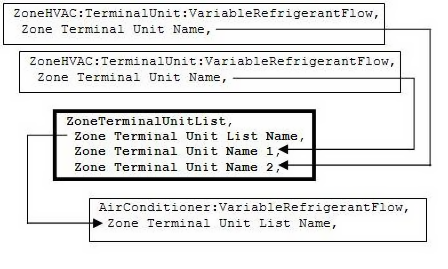
\includegraphics[width=0.9\textwidth, height=0.9\textheight, keepaspectratio=true]{media/image313.png}
\caption{Zone Terminal Unit List Diagram \protect \label{fig:zone-terminal-unit-list-diagram}}
\end{figure}
\subsubsection{Inputs}\label{inputs-2-044}

\paragraph{Field: Zone Terminal List Name}\label{field-zone-terminal-list-name}

This alpha field specifies the name of the zone terminal unit list. This name must be specified in the \hyperref[airconditionervariablerefrigerantflow]{AirConditioner:VariableRefrigerantFlow} object.

\paragraph{Field: Zone Terminal Unit Name \textless{}x\textgreater{}}\label{field-zone-terminal-unit-name-x}

This alpha field defines the name of the zone terminal unit used in a variable refrigerant air conditioner. The zone terminal unit must be connected to a zone using the \hyperref[zonehvacequipmentconnections]{ZoneHVAC:EquipmentConnections} object. The terminal unit air inlet node is the same name as a zone exhaust node. The terminal unit air outlet node is the same name as a zone inlet node. The IDD is supplied with 20 fields for this.~ The object is extensible and you can change the IDD by adding more fields or, if you are using text editor for your input file, just add to the list of names.

Following is an example input for a ZoneTerminalUnitList object.

\begin{lstlisting}

ZoneTerminalUnitList,
     VRF Heat Pump TU List, !- Zone Terminal Unit List Name
     TU3,                   !- Zone Terminal Unit Name 1
     TU4,                   !- Zone Terminal Unit Name 2
     TU1,                   !- Zone Terminal Unit Name 3
     TU2,                   !- Zone Terminal Unit Name 4
     TU5;                   !- Zone Terminal Unit Name 5
\end{lstlisting}